% Options for packages loaded elsewhere
\PassOptionsToPackage{unicode}{hyperref}
\PassOptionsToPackage{hyphens}{url}
\PassOptionsToPackage{dvipsnames,svgnames,x11names}{xcolor}
%
\documentclass[
  letterpaper,
  DIV=11,
  numbers=noendperiod]{scrreprt}

\usepackage{amsmath,amssymb}
\usepackage{iftex}
\ifPDFTeX
  \usepackage[T1]{fontenc}
  \usepackage[utf8]{inputenc}
  \usepackage{textcomp} % provide euro and other symbols
\else % if luatex or xetex
  \usepackage{unicode-math}
  \defaultfontfeatures{Scale=MatchLowercase}
  \defaultfontfeatures[\rmfamily]{Ligatures=TeX,Scale=1}
\fi
\usepackage{lmodern}
\ifPDFTeX\else  
    % xetex/luatex font selection
\fi
% Use upquote if available, for straight quotes in verbatim environments
\IfFileExists{upquote.sty}{\usepackage{upquote}}{}
\IfFileExists{microtype.sty}{% use microtype if available
  \usepackage[]{microtype}
  \UseMicrotypeSet[protrusion]{basicmath} % disable protrusion for tt fonts
}{}
\makeatletter
\@ifundefined{KOMAClassName}{% if non-KOMA class
  \IfFileExists{parskip.sty}{%
    \usepackage{parskip}
  }{% else
    \setlength{\parindent}{0pt}
    \setlength{\parskip}{6pt plus 2pt minus 1pt}}
}{% if KOMA class
  \KOMAoptions{parskip=half}}
\makeatother
\usepackage{xcolor}
\setlength{\emergencystretch}{3em} % prevent overfull lines
\setcounter{secnumdepth}{5}
% Make \paragraph and \subparagraph free-standing
\ifx\paragraph\undefined\else
  \let\oldparagraph\paragraph
  \renewcommand{\paragraph}[1]{\oldparagraph{#1}\mbox{}}
\fi
\ifx\subparagraph\undefined\else
  \let\oldsubparagraph\subparagraph
  \renewcommand{\subparagraph}[1]{\oldsubparagraph{#1}\mbox{}}
\fi

\usepackage{color}
\usepackage{fancyvrb}
\newcommand{\VerbBar}{|}
\newcommand{\VERB}{\Verb[commandchars=\\\{\}]}
\DefineVerbatimEnvironment{Highlighting}{Verbatim}{commandchars=\\\{\}}
% Add ',fontsize=\small' for more characters per line
\usepackage{framed}
\definecolor{shadecolor}{RGB}{241,243,245}
\newenvironment{Shaded}{\begin{snugshade}}{\end{snugshade}}
\newcommand{\AlertTok}[1]{\textcolor[rgb]{0.68,0.00,0.00}{#1}}
\newcommand{\AnnotationTok}[1]{\textcolor[rgb]{0.37,0.37,0.37}{#1}}
\newcommand{\AttributeTok}[1]{\textcolor[rgb]{0.40,0.45,0.13}{#1}}
\newcommand{\BaseNTok}[1]{\textcolor[rgb]{0.68,0.00,0.00}{#1}}
\newcommand{\BuiltInTok}[1]{\textcolor[rgb]{0.00,0.23,0.31}{#1}}
\newcommand{\CharTok}[1]{\textcolor[rgb]{0.13,0.47,0.30}{#1}}
\newcommand{\CommentTok}[1]{\textcolor[rgb]{0.37,0.37,0.37}{#1}}
\newcommand{\CommentVarTok}[1]{\textcolor[rgb]{0.37,0.37,0.37}{\textit{#1}}}
\newcommand{\ConstantTok}[1]{\textcolor[rgb]{0.56,0.35,0.01}{#1}}
\newcommand{\ControlFlowTok}[1]{\textcolor[rgb]{0.00,0.23,0.31}{#1}}
\newcommand{\DataTypeTok}[1]{\textcolor[rgb]{0.68,0.00,0.00}{#1}}
\newcommand{\DecValTok}[1]{\textcolor[rgb]{0.68,0.00,0.00}{#1}}
\newcommand{\DocumentationTok}[1]{\textcolor[rgb]{0.37,0.37,0.37}{\textit{#1}}}
\newcommand{\ErrorTok}[1]{\textcolor[rgb]{0.68,0.00,0.00}{#1}}
\newcommand{\ExtensionTok}[1]{\textcolor[rgb]{0.00,0.23,0.31}{#1}}
\newcommand{\FloatTok}[1]{\textcolor[rgb]{0.68,0.00,0.00}{#1}}
\newcommand{\FunctionTok}[1]{\textcolor[rgb]{0.28,0.35,0.67}{#1}}
\newcommand{\ImportTok}[1]{\textcolor[rgb]{0.00,0.46,0.62}{#1}}
\newcommand{\InformationTok}[1]{\textcolor[rgb]{0.37,0.37,0.37}{#1}}
\newcommand{\KeywordTok}[1]{\textcolor[rgb]{0.00,0.23,0.31}{#1}}
\newcommand{\NormalTok}[1]{\textcolor[rgb]{0.00,0.23,0.31}{#1}}
\newcommand{\OperatorTok}[1]{\textcolor[rgb]{0.37,0.37,0.37}{#1}}
\newcommand{\OtherTok}[1]{\textcolor[rgb]{0.00,0.23,0.31}{#1}}
\newcommand{\PreprocessorTok}[1]{\textcolor[rgb]{0.68,0.00,0.00}{#1}}
\newcommand{\RegionMarkerTok}[1]{\textcolor[rgb]{0.00,0.23,0.31}{#1}}
\newcommand{\SpecialCharTok}[1]{\textcolor[rgb]{0.37,0.37,0.37}{#1}}
\newcommand{\SpecialStringTok}[1]{\textcolor[rgb]{0.13,0.47,0.30}{#1}}
\newcommand{\StringTok}[1]{\textcolor[rgb]{0.13,0.47,0.30}{#1}}
\newcommand{\VariableTok}[1]{\textcolor[rgb]{0.07,0.07,0.07}{#1}}
\newcommand{\VerbatimStringTok}[1]{\textcolor[rgb]{0.13,0.47,0.30}{#1}}
\newcommand{\WarningTok}[1]{\textcolor[rgb]{0.37,0.37,0.37}{\textit{#1}}}

\providecommand{\tightlist}{%
  \setlength{\itemsep}{0pt}\setlength{\parskip}{0pt}}\usepackage{longtable,booktabs,array}
\usepackage{calc} % for calculating minipage widths
% Correct order of tables after \paragraph or \subparagraph
\usepackage{etoolbox}
\makeatletter
\patchcmd\longtable{\par}{\if@noskipsec\mbox{}\fi\par}{}{}
\makeatother
% Allow footnotes in longtable head/foot
\IfFileExists{footnotehyper.sty}{\usepackage{footnotehyper}}{\usepackage{footnote}}
\makesavenoteenv{longtable}
\usepackage{graphicx}
\makeatletter
\def\maxwidth{\ifdim\Gin@nat@width>\linewidth\linewidth\else\Gin@nat@width\fi}
\def\maxheight{\ifdim\Gin@nat@height>\textheight\textheight\else\Gin@nat@height\fi}
\makeatother
% Scale images if necessary, so that they will not overflow the page
% margins by default, and it is still possible to overwrite the defaults
% using explicit options in \includegraphics[width, height, ...]{}
\setkeys{Gin}{width=\maxwidth,height=\maxheight,keepaspectratio}
% Set default figure placement to htbp
\makeatletter
\def\fps@figure{htbp}
\makeatother
\newlength{\cslhangindent}
\setlength{\cslhangindent}{1.5em}
\newlength{\csllabelwidth}
\setlength{\csllabelwidth}{3em}
\newlength{\cslentryspacingunit} % times entry-spacing
\setlength{\cslentryspacingunit}{\parskip}
\newenvironment{CSLReferences}[2] % #1 hanging-ident, #2 entry spacing
 {% don't indent paragraphs
  \setlength{\parindent}{0pt}
  % turn on hanging indent if param 1 is 1
  \ifodd #1
  \let\oldpar\par
  \def\par{\hangindent=\cslhangindent\oldpar}
  \fi
  % set entry spacing
  \setlength{\parskip}{#2\cslentryspacingunit}
 }%
 {}
\usepackage{calc}
\newcommand{\CSLBlock}[1]{#1\hfill\break}
\newcommand{\CSLLeftMargin}[1]{\parbox[t]{\csllabelwidth}{#1}}
\newcommand{\CSLRightInline}[1]{\parbox[t]{\linewidth - \csllabelwidth}{#1}\break}
\newcommand{\CSLIndent}[1]{\hspace{\cslhangindent}#1}

\KOMAoption{captions}{tableheading}
\makeatletter
\@ifpackageloaded{tcolorbox}{}{\usepackage[skins,breakable]{tcolorbox}}
\@ifpackageloaded{fontawesome5}{}{\usepackage{fontawesome5}}
\definecolor{quarto-callout-color}{HTML}{909090}
\definecolor{quarto-callout-note-color}{HTML}{0758E5}
\definecolor{quarto-callout-important-color}{HTML}{CC1914}
\definecolor{quarto-callout-warning-color}{HTML}{EB9113}
\definecolor{quarto-callout-tip-color}{HTML}{00A047}
\definecolor{quarto-callout-caution-color}{HTML}{FC5300}
\definecolor{quarto-callout-color-frame}{HTML}{acacac}
\definecolor{quarto-callout-note-color-frame}{HTML}{4582ec}
\definecolor{quarto-callout-important-color-frame}{HTML}{d9534f}
\definecolor{quarto-callout-warning-color-frame}{HTML}{f0ad4e}
\definecolor{quarto-callout-tip-color-frame}{HTML}{02b875}
\definecolor{quarto-callout-caution-color-frame}{HTML}{fd7e14}
\makeatother
\makeatletter
\makeatother
\makeatletter
\@ifpackageloaded{bookmark}{}{\usepackage{bookmark}}
\makeatother
\makeatletter
\@ifpackageloaded{caption}{}{\usepackage{caption}}
\AtBeginDocument{%
\ifdefined\contentsname
  \renewcommand*\contentsname{Table of contents}
\else
  \newcommand\contentsname{Table of contents}
\fi
\ifdefined\listfigurename
  \renewcommand*\listfigurename{List of Figures}
\else
  \newcommand\listfigurename{List of Figures}
\fi
\ifdefined\listtablename
  \renewcommand*\listtablename{List of Tables}
\else
  \newcommand\listtablename{List of Tables}
\fi
\ifdefined\figurename
  \renewcommand*\figurename{Figure}
\else
  \newcommand\figurename{Figure}
\fi
\ifdefined\tablename
  \renewcommand*\tablename{Table}
\else
  \newcommand\tablename{Table}
\fi
}
\@ifpackageloaded{float}{}{\usepackage{float}}
\floatstyle{ruled}
\@ifundefined{c@chapter}{\newfloat{codelisting}{h}{lop}}{\newfloat{codelisting}{h}{lop}[chapter]}
\floatname{codelisting}{Listing}
\newcommand*\listoflistings{\listof{codelisting}{List of Listings}}
\makeatother
\makeatletter
\@ifpackageloaded{caption}{}{\usepackage{caption}}
\@ifpackageloaded{subcaption}{}{\usepackage{subcaption}}
\makeatother
\makeatletter
\@ifpackageloaded{tcolorbox}{}{\usepackage[skins,breakable]{tcolorbox}}
\makeatother
\makeatletter
\@ifundefined{shadecolor}{\definecolor{shadecolor}{rgb}{.97, .97, .97}}
\makeatother
\makeatletter
\makeatother
\makeatletter
\makeatother
\ifLuaTeX
  \usepackage{selnolig}  % disable illegal ligatures
\fi
\IfFileExists{bookmark.sty}{\usepackage{bookmark}}{\usepackage{hyperref}}
\IfFileExists{xurl.sty}{\usepackage{xurl}}{} % add URL line breaks if available
\urlstyle{same} % disable monospaced font for URLs
\hypersetup{
  pdftitle={The Mini Buoy Handbook},
  pdfauthor={Thorsten Balke; Cai Ladd; Marie-Christin Wimmler; Alejandra Vovides},
  colorlinks=true,
  linkcolor={blue},
  filecolor={Maroon},
  citecolor={Blue},
  urlcolor={Blue},
  pdfcreator={LaTeX via pandoc}}

\title{The Mini Buoy Handbook}
\usepackage{etoolbox}
\makeatletter
\providecommand{\subtitle}[1]{% add subtitle to \maketitle
  \apptocmd{\@title}{\par {\large #1 \par}}{}{}
}
\makeatother
\subtitle{Assessing hydrodynamics in intertidal environments}
\author{Thorsten Balke \and Cai Ladd \and Marie-Christin
Wimmler \and Alejandra Vovides}
\date{2023-04-19}

\begin{document}
\maketitle
\ifdefined\Shaded\renewenvironment{Shaded}{\begin{tcolorbox}[sharp corners, interior hidden, frame hidden, enhanced, borderline west={3pt}{0pt}{shadecolor}, boxrule=0pt, breakable]}{\end{tcolorbox}}\fi

\renewcommand*\contentsname{Table of contents}
{
\hypersetup{linkcolor=}
\setcounter{tocdepth}{2}
\tableofcontents
}
\bookmarksetup{startatroot}

\hypertarget{preface}{%
\chapter*{Preface}\label{preface}}
\addcontentsline{toc}{chapter}{Preface}

\markboth{Preface}{Preface}

The `Mini Buoy' is an applied research tool to measure inundation
duration, current velocity, and wave orbital velocity in shallow coastal
settings using accelerometer technology. As a low cost and open-source
solution, Mini Buoys and the associated App are a useful alternative to
conventional hydrodynamic sensors.

This guide provides an overview of how the Mini Buoy works, how to
configure and deploy them, and how to analyse the data\footnote{The
  MSR145W B4 is a standalone accelerometer with integrated rechargeable
  lithium ion battery and memory in a waterproof seal. Acceleration is
  measured along the y-axis.}.

\bookmarksetup{startatroot}

\hypertarget{sec-intro}{%
\chapter{Introduction}\label{sec-intro}}

There are presently three Mini Buoy designs featured in this handbook,
each with their own strengths and limitations:

\begin{itemize}
\tightlist
\item
  \textbf{B4} is the original Mini Buoy design featured in Balke et
  al.~(2021) that contains an MSR145 B4 acceleration data logger inside
  a self-standing centrifuge tube attached to an anchor via a fishing
  swivel. The B4 measures inundation duration and current velocity
  only.\\
\item
  \textbf{B4+} is a more durable version of the original Mini Buoy ideal
  for long term deployments. The B4+ has a UV-resistant casing without
  the skirt and a metal eye bolt connected to a mooring by crimped
  fishing line rings. In addition to measuring inundation duration and
  current velocity, the B4+ has been calibrated to measure wave orbital
  velocities. Whilst the durability and functionality may be improved,
  the B4+ requires more effort to assemble.
\item
  \textbf{Pendant} is an integrated accelerometer data logger, float,
  and anchor point, attached to a pole by a fishing swivel. The Pendant
  is less expensive and easier to assemble than the B4 and B4+, however
  memory capacity and sampling rates are lower. Because of the low
  sampling rate, the Pendant is unstable for measuring wave orbital
  velocity.
\end{itemize}

\begin{figure}

{\centering 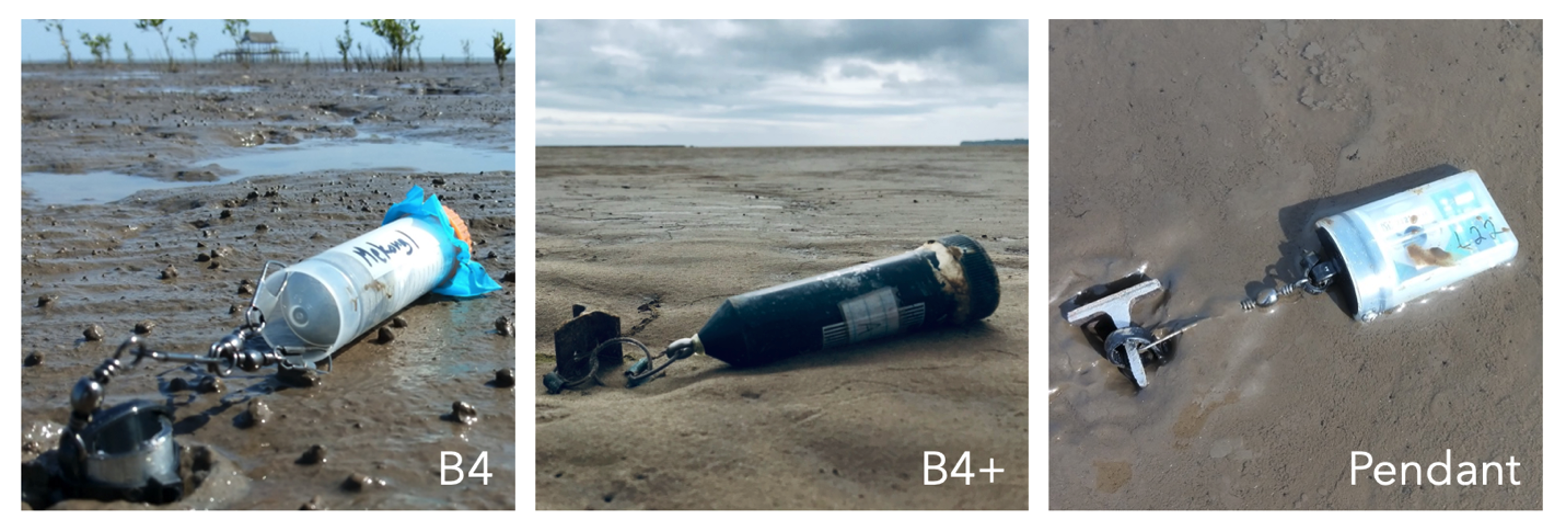
\includegraphics{chapters/figs/MiniBuoysPhotos.png}

}

\end{figure}

Once assembled, Mini Buoys can be used in single, comparative, or
multiple deployments for purposes of habitat restoration potential
mapping, flood risk monitoring, and citizen science engagement.

\hypertarget{tbl-1}{}
\begin{longtable}[]{@{}
  >{\raggedright\arraybackslash}p{(\columnwidth - 6\tabcolsep) * \real{0.3210}}
  >{\centering\arraybackslash}p{(\columnwidth - 6\tabcolsep) * \real{0.2222}}
  >{\centering\arraybackslash}p{(\columnwidth - 6\tabcolsep) * \real{0.2222}}
  >{\centering\arraybackslash}p{(\columnwidth - 6\tabcolsep) * \real{0.2346}}@{}}
\caption{\label{tbl-1}Comparison of each Mini Buoy
design.}\tabularnewline
\toprule\noalign{}
\begin{minipage}[b]{\linewidth}\raggedright
\end{minipage} & \begin{minipage}[b]{\linewidth}\centering
B4
\end{minipage} & \begin{minipage}[b]{\linewidth}\centering
B4+
\end{minipage} & \begin{minipage}[b]{\linewidth}\centering
Pendant
\end{minipage} \\
\midrule\noalign{}
\endfirsthead
\toprule\noalign{}
\begin{minipage}[b]{\linewidth}\raggedright
\end{minipage} & \begin{minipage}[b]{\linewidth}\centering
B4
\end{minipage} & \begin{minipage}[b]{\linewidth}\centering
B4+
\end{minipage} & \begin{minipage}[b]{\linewidth}\centering
Pendant
\end{minipage} \\
\midrule\noalign{}
\endhead
\bottomrule\noalign{}
\endlastfoot
Cost & £430 & £430 & £120 \\
Total weight & 42.3 g & 60.0 g & 19.9 g \\
Sensing height above bed & 16 cm & 16 cm & 10.5 cm \\
Deployment duration & 1 sec: 25 days & 1 sec: 25 days & 2 min:
\textbf{XXX} days \\
Deployment duration & 5 sec: 125 days & 5 sec: 125 days & 6 min:
\textbf{XXX} days \\
Deployment duration & 10 sec: 170 days & 10 sec: 170 days & 10 min:
\textbf{XXX} days \\
Currents detection limit & 4.3 cm/s & 1.8 cm/s & 4.9 cm/s \\
Currents accuracy & ±18.9 cm/s & ±13.8 cm/s & ±2.20 cm/s \\
Waves detection range & - & 0.0 cm/s & - \\
Waves accuracy & - & \textbf{±17.X cm/s} & - \\
Compatibility & Windows & Windows & Windows and macOS \\
\end{longtable}

\hypertarget{operating-principles}{%
\section{Operating principles}\label{operating-principles}}

Inundation duration, current velocity, and wave orbital velocity
parameters can all be derived from acceleration data.

For an accelerometer mounted in a tethered float, the change in tilt
from 0 to 90° indicates a change in the position of the device from
lying horizontally on the tidal flat to floating vertically in the water
column as the tide comes in. A return of the tilt to 0° indicates the
tide has retreated and the Mini Buoy is once again lying flat. The time
when the Mini Buoy deviated from the horizontal position gives the
inundation duration of the tide (Figure A below). When the Mini Buoy is
fully inundated, any tilting away from the vertical position is caused
by a current pushing against the buoy. The stronger the current, the
stronger the tilt (Figure B below). When waves pass over the Mini Buoy,
they cause it to wobble. Moving standard deviation in the tilt over a
sufficient time window captures the average wave orbital velocity near
the bed. The greater the standard deviation, the greater the wave
orbital velocity (Figure C below).

\begin{figure}

{\centering 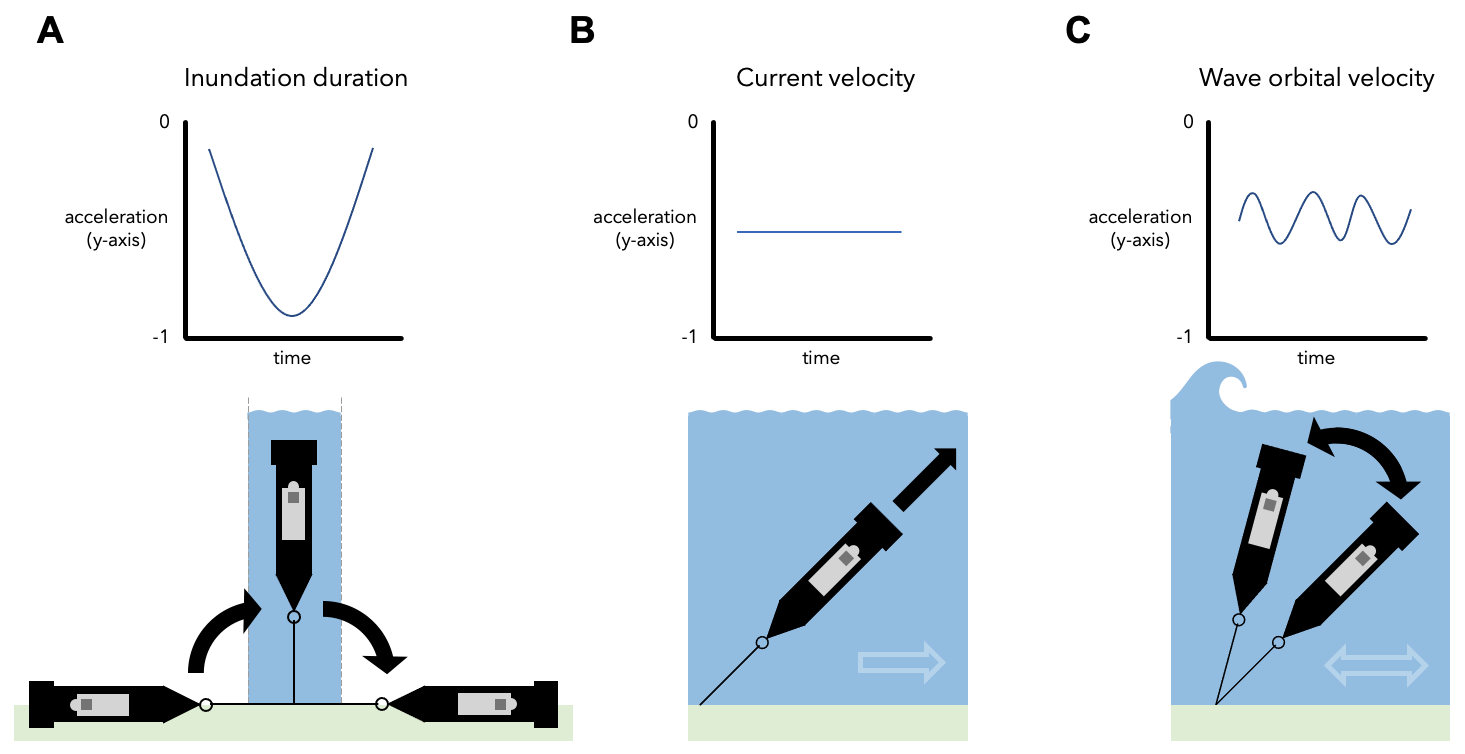
\includegraphics{chapters/figs/OperatingPrinciples.png}

}

\end{figure}

Testing has shown that inundation status is correctly identified at
rates of 87-99\% across all designs. To identify the inundation status
of a Mini Buoy from acceleration data, a classifier algorithm (Quadratic
Discriminant Analysis) differentiates inundated and non-inundated cases
from the median and standard deviation in tilt; median and standard
deviation values are near zero for a Mini Buoy at rest, and are larger
when a Mini Buoy is inundated:

\begin{figure}

{\centering 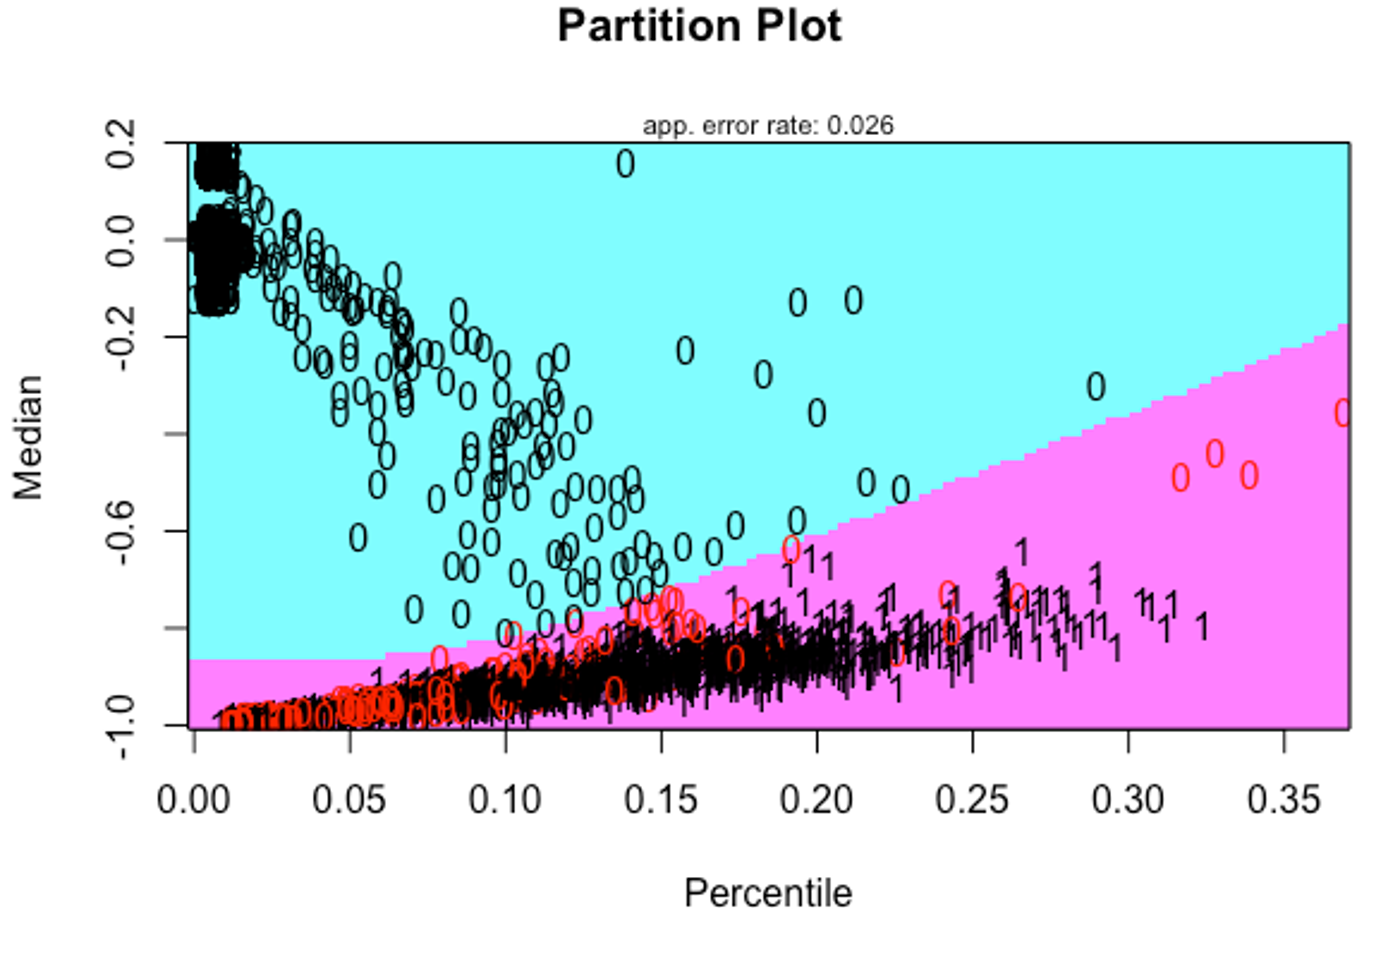
\includegraphics[width=0.7\textwidth,height=\textheight]{chapters/figs/QDA.png}

}

\end{figure}

Partially inundated cases are then identified using an abrupt shift
detection algorithm (Boulton, 2022) that searches for the continuous
change in Mini Buoy tilt from 0 to \textasciitilde90° at the start of
the flood tide and \textasciitilde90 to 0° at the end of the ebb tide,
characteristic of partially inundated cases before/after peak flood/ebb
currents:

\begin{figure}

{\centering 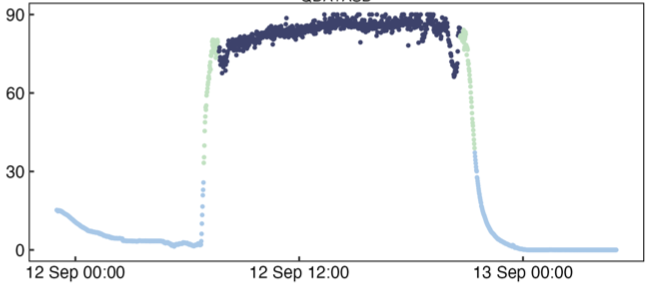
\includegraphics[width=0.7\textwidth,height=\textheight]{chapters/figs/ASD.png}

}

\end{figure}

Conversion from tilt to velocity has been done by deploying each Mini
Buoy design adjacent to hydrographic sensors that measure water velocity
directly. Current velocities as low as 0.01 m/s and as high as 0.75 m/s
can be detected with good accuracy (Figures A-C below). The B4+ is
reasonable at measuring wave orbital velocities between 0 and 0.2 m/s
(Figure D below).

\begin{figure}

{\centering 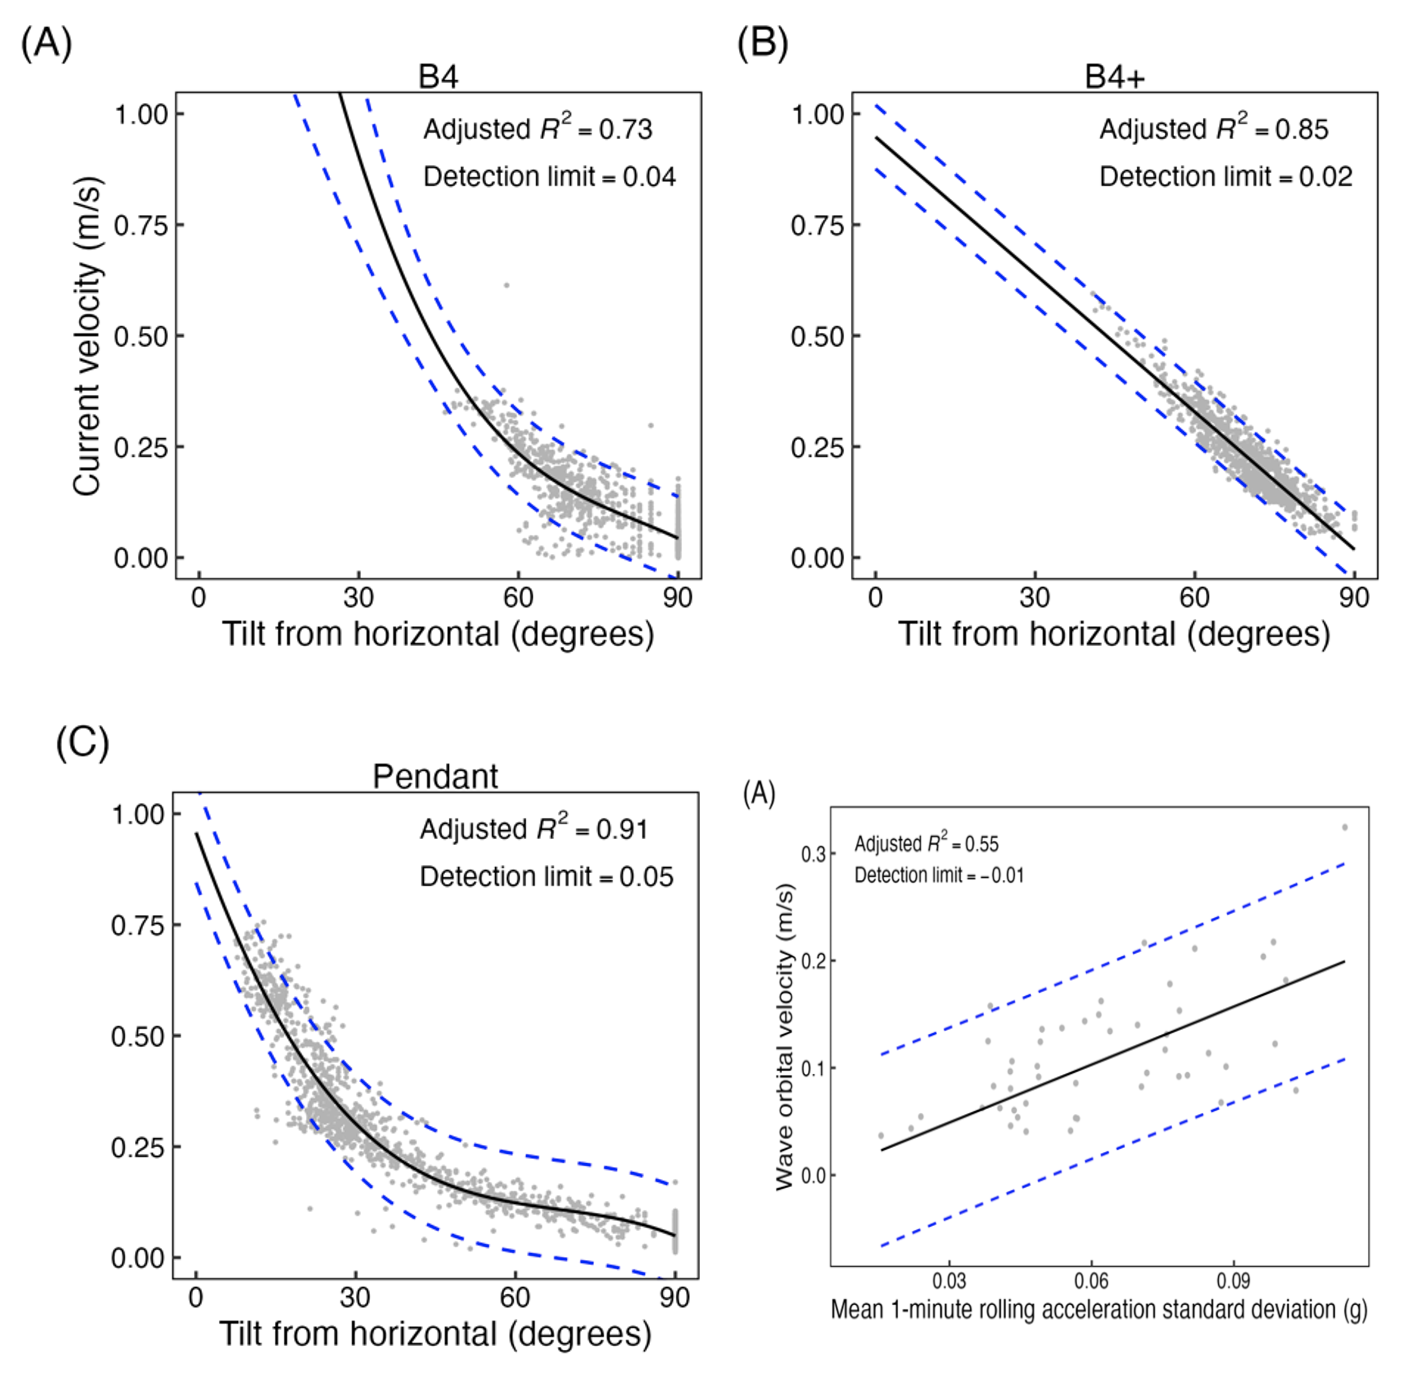
\includegraphics[width=0.7\textwidth,height=\textheight]{chapters/figs/CalibrationCurves.png}

}

\end{figure}

A comprehensive description of the Mini Buoy calibrations is given in
Ladd et al.~(2023).

\bookmarksetup{startatroot}

\hypertarget{assembly}{%
\chapter{Assembly}\label{assembly}}

Depending on their requirements, the user has a choice of three Mini
Buoy designs for measuring hydrodynamics (see Chapter~\ref{sec-intro}).
In the following steps, we provide instructions for the assembly of each
design.

\hypertarget{b4}{%
\section{B4}\label{b4}}

The B4 is a transparent and self-standing centrifuge tube with an
MSR145W B4\footnote{The MSR145W B4 is a standalone accelerometer with
  integrated rechargeable lithium ion battery and memory in a waterproof
  seal. Acceleration is measured along the y-axis.} acceleration logger
sealed inside and supported by floral foam. The tube is tethered to an
anchor using fishing swivels attached through two holes in the
centrifuge tube skirt. To build a B4, first gather the following
equipment:

\begin{itemize}
\tightlist
\item
  50 mL clear self-standing centrifuge tube
\item
  Label
\item
  Floral foam
\item
  \href{https://www.msr.ch/en/product/msr145/}{MSR145W B4} acceleration
  data logger
\item
  Silicone sealant
\item
  Drill with a 4 mm dowel bit
\item
  3 × 5 cm (1.1 g) fishing swivels
\end{itemize}

To assemble the B4 Mini Buoy:

\begin{enumerate}
\def\labelenumi{\arabic{enumi}.}
\tightlist
\item
  Place a label inside the centrifuge tube, with the text legible
  through the plastic, indicating the owner, a ``do not remove'' notice,
  and contact details
\item
  Insert a 3 cm cylinder of floral foam into the centrifuge tube. This
  ensures the logger is positioned at the top of the tube
\item
  Roughly cut a 5 cm cylinder of floral foam with matching diameter of
  the centrifuge tube and cut down the middle
\item
  Place both halves around the configured MSR145W B4 acceleration data
  logger, then gently push the logger into the centrifuge tube with the
  PC connector facing outwards. The floral foam will prevent the logger
  from moving inside the tube
\item
  Apply silicone sealant around the screw thread of the centrifuge tube
  and fasten the cap
\item
  Apply more sealant along the rim of the centrifuge cap if necessary
\item
  Drill two holes at opposite ends through the centrifuge tube skirt 5
  mm from the bottom
\item
  Fix two fishing swivels through each hole, and connect both to another
  swivel as shown:
\end{enumerate}

\begin{figure}

{\centering 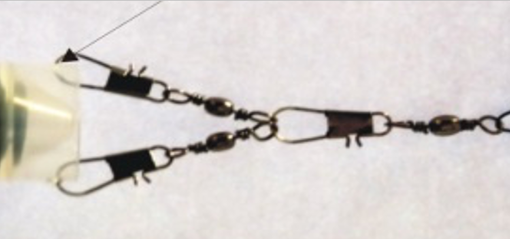
\includegraphics[width=0.7\textwidth,height=\textheight]{chapters/figs/B4FishingSwivel.png}

}

\end{figure}

\hypertarget{b4-1}{%
\section{B4+}\label{b4-1}}

The B4+ almost identical in design to the B4, with some modifications:
the centrifuge tube is UV-resistant without a skirt, an eye bolt and
fishing line rings are fitted to provide more durability, and steel shot
is added to the tube to increase sensitivity to current and wave action.
Gather the following equipment to assemble the B4+:

\begin{itemize}
\tightlist
\item
  50 mL UV-blocking centrifuge tube
\item
  Sand paper
\item
  Drill with a 4 mm dowel bit
\item
  M4 Eye bolt and nut
\item
  M4 rubber washer
\item
  M4 long socket
\item
  Epoxy glue
\item
  M32 O-rings
\item
  20 g lead shot weight
\item
  Floral foam
\item
  Waterproof label
\item
  250 lb / 113 kg nylon coated 1×7 steel strand fishing line
\item
  Single barrel copper/nickel crimp sleeves (the sleeves should be rated
  to correctly fit the fishing line)
\item
  Crimp tool with cutter (the tool should be rated to correctly crimp
  the sleeves)
\item
  MSR145W B4 acceleration data logger
\item
  Silicone sealant
\end{itemize}

To assemble the B4+ Mini Buoy:

\begin{enumerate}
\def\labelenumi{\arabic{enumi}.}
\tightlist
\item
  Abrade the bottom of the centrifuge tube (this removes any lubricant
  on the tube and creates a better surface for the epoxy glue to bond
  with)
\item
  Drill a 4 mm hole in the bottom of the centrifuge tube
\item
  Thread the eye bolt through the hole
\item
  Place the rubber washer over the eye bolt thread from inside the tube
\item
  Dab some epoxy glue around the eye bolt (inside and out) to seal the
  hole
\item
  Secure the nut in place using the long socket
\end{enumerate}

\begin{figure}

{\centering 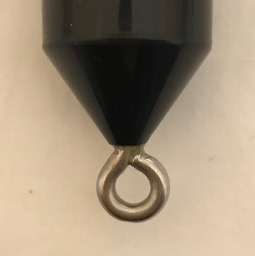
\includegraphics[width=0.7\textwidth,height=\textheight]{chapters/figs/B4pEyeHook.jpg}

}

\end{figure}

\begin{enumerate}
\def\labelenumi{\arabic{enumi}.}
\setcounter{enumi}{6}
\tightlist
\item
  To ensure watertightness, install a rubber o-ring around the inside
  lip of the lid using tweezers as shown:
\end{enumerate}

\begin{figure}

{\centering 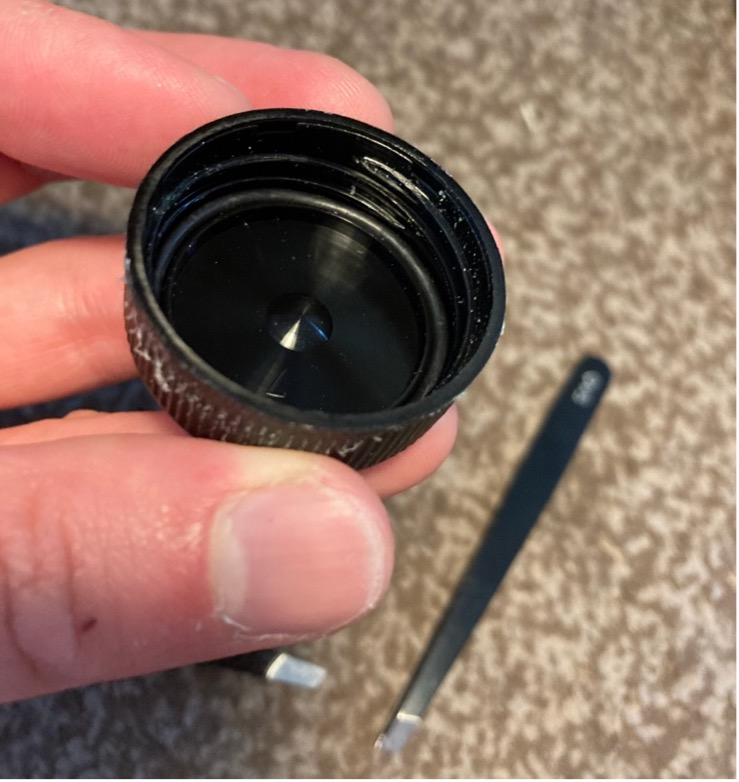
\includegraphics[width=0.7\textwidth,height=\textheight]{chapters/figs/B4pLidSeal.jpg}

}

\end{figure}

\begin{enumerate}
\def\labelenumi{\arabic{enumi}.}
\setcounter{enumi}{7}
\tightlist
\item
  Pour 20 g of steel shot into the tube. The shot reduces the buoyancy
  of the Mini Buoy, making it less stable in the water column. This has
  been shown to improve the accelerometer sensitivity
\item
  Cut a 3 cm length cylinder from the floral foam that will fit
  comfortably into the tube
\item
  Insert the floral foam cylinder into the tube. This holds the steel
  shot in place and ensures the logger is positioned at the top of the
  tube\\
\item
  Attach a waterproof label onto the centrifuge tube indicating the
  owner, a ``do not remove'' notice, and contact details
\item
  Thread the fishing line through a crimp sleeve and loop the fishing
  line back on itself to form a ring of \textasciitilde2 cm diameter
\item
  Crimp the sleeve so it fits tightly around the fishing line
\item
  Thread another fishing line through a new crimp sleeve, then through
  the eye bolt and first fishing line ring
\item
  Adjust the diameter of the ring so the total chain length is 4 cm,
  then crimp (the B4+ has been calibrated to measure hydrodynamics 4 cm
  above the tidal flat). The tether should look as follows:
\end{enumerate}

\begin{figure}

{\centering 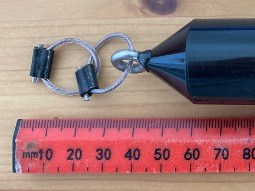
\includegraphics[width=0.7\textwidth,height=\textheight]{chapters/figs/B4pFishingLineChain.jpg}

}

\end{figure}

\begin{enumerate}
\def\labelenumi{\arabic{enumi}.}
\setcounter{enumi}{15}
\tightlist
\item
  Roughly cut a 5 cm cylinder of floral foam with matching diameter of
  the centrifuge tube and cut down the middle
\item
  Place both halves around the configured MSR145W B4 acceleration data
  logger, then gently push the logger into the centrifuge tube with the
  PC connector facing upright. The floral foam will prevent the logger
  from moving inside the tube
\item
  Apply silicone sealant around the screw thread of the centrifuge tube
  and fasten the tube cap
\item
  Apply more sealant along the rim of the centrifuge cap
\end{enumerate}

\hypertarget{pendant}{%
\section{Pendant}\label{pendant}}

The Pendant\footnote{The Pendant G Data Logger is a standalone
  accelerometer with a coin cell battery and memory in a waterproof
  seal. Acceleration is measured along the x-axis.} can be directly
tethered to a pole in the ground using fishing swivels as the logger
itself is buoyant and waterproof. Gather the following equipment:

\begin{itemize}
\tightlist
\item
  \href{https://www.onsetcomp.com/products/data-loggers/ua-004-64/}{HOBO
  Pendant G} acceleration data logger
\item
  \href{https://www.onsetcomp.com/products/communications/base-u-4}{HOBO
  Optic USB Base Station} necessary for connecting the logger to the PC
\item
  5 cm (1.1 g) fishing swivel
\end{itemize}

To assemble the Pendant Mini Buoy, simply attach the fishing swivel to
the anchor point on the Pendant logger as shown:

\begin{figure}

{\centering 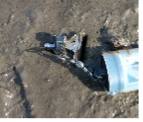
\includegraphics[width=0.7\textwidth,height=\textheight]{chapters/figs/PendantTether.jpg}

}

\end{figure}

\bookmarksetup{startatroot}

\hypertarget{configuration}{%
\chapter{Configuration}\label{configuration}}

Prior to each deployment of the Mini Buoy, the data logger will need to
be fully charged, have a full memory, and be correctly configured
according to the user's requirements. The following section describes
how to configure the MSR145W B4 (used in both the B4 and B4+ Mini Buoy
designs) and HOBO Pendant G acceleration data loggers.

\hypertarget{msr145}{%
\section{MSR145}\label{msr145}}

The MSR145W B4 comes with a USB charging cable. Free software to
configure the logger can be downloaded
\href{https://www.msr.ch/en/support/msr-pc-software-standard/}{here}. At
present, the logger is only compatible with a Windows PC. To configure
the MSR145W B4:

\begin{enumerate}
\def\labelenumi{\arabic{enumi}.}
\tightlist
\item
  Download and install the
  \href{https://www.msr.ch/en/support/pcsoftware/}{MSR software}
\item
  Connect a logger to a Windows PC. A yellow LED will light up on the
  logger, indicating the internal battery is being charged. The light
  will extinguish once the battery is fully charged
\item
  Open the MSR software
\item
  Double-click \texttt{Setup}
\end{enumerate}

\begin{figure}

{\centering 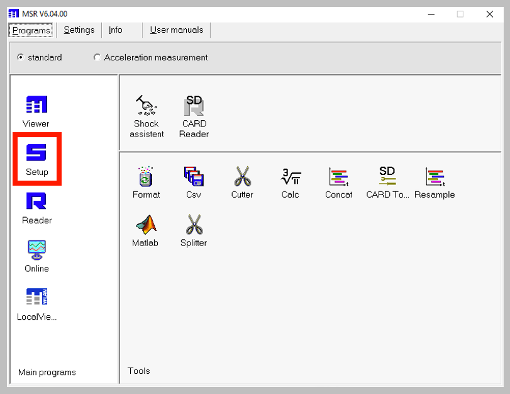
\includegraphics[width=0.7\textwidth,height=\textheight]{chapters/figs/MSRStep1.png}

}

\end{figure}

\begin{enumerate}
\def\labelenumi{\arabic{enumi}.}
\setcounter{enumi}{4}
\tightlist
\item
  Select the \texttt{Format\ memory} tab
\item
  Click \texttt{Format}. This will delete any data stored on the logger
\end{enumerate}

\begin{figure}

{\centering 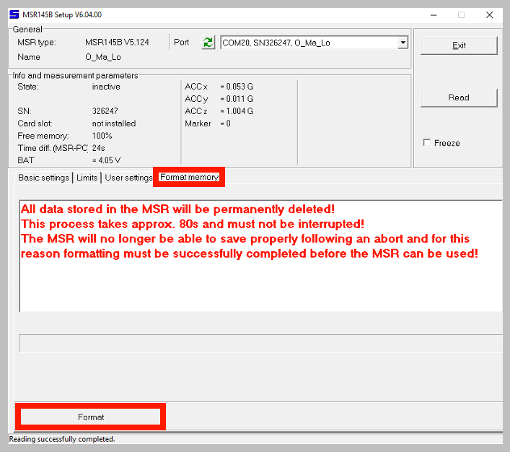
\includegraphics[width=0.7\textwidth,height=\textheight]{chapters/figs/MSRStep2.png}

}

\end{figure}

\begin{enumerate}
\def\labelenumi{\arabic{enumi}.}
\setcounter{enumi}{6}
\tightlist
\item
  Once formatting is complete, select the \texttt{User\ settings} tab
\item
  Set the acceleration sensor measure range to \texttt{2G}
\item
  You can define a name for the logger under \texttt{Name\ of\ logger}
\item
  Click \texttt{Write\ user\ settings}
\end{enumerate}

\begin{figure}

{\centering 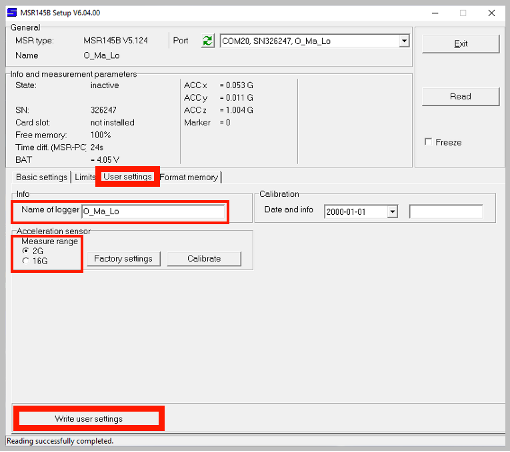
\includegraphics[width=0.7\textwidth,height=\textheight]{chapters/figs/MSRStep3.png}

}

\end{figure}

\begin{enumerate}
\def\labelenumi{\arabic{enumi}.}
\setcounter{enumi}{10}
\tightlist
\item
  Check the \texttt{limits} box
\item
  Select the \texttt{Limits} tab. We can use limits to effectively
  disable the X and Y sensors by setting unrealistically high
  acceleration limits. This will allow your logger to store more Y
  acceleration data.
\item
  For ACC x and ACC z channels, select
  \texttt{\textless{}L1\ or\ \textgreater{}L2,\ (Shock)} from the record
  limit drop-down menu
\item
  Set the corresponding \texttt{Limit\ L1} to -999 and
  \texttt{Limit\ L2} to +999. The MSR software will default to the
  maximum possible range
\item
  Make sure there are no limits set on the ACC y channel by selecting
  \texttt{inactive} from the record limit drop-down menu
\item
  Click the \texttt{\textless{}} button
\end{enumerate}

\begin{figure}

{\centering 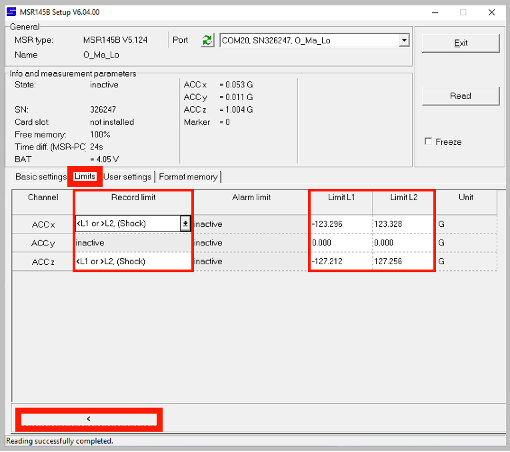
\includegraphics[width=0.7\textwidth,height=\textheight]{chapters/figs/MSRStep4.png}

}

\end{figure}

\begin{enumerate}
\def\labelenumi{\arabic{enumi}.}
\setcounter{enumi}{16}
\tightlist
\item
  Select the \texttt{Basic\ settings} tab
\item
  Under \texttt{Sensors}, select \texttt{t1} from the
  \texttt{ACC\ x,\ y,\ z} drop-down menu
\item
  Under \texttt{Main\ storage\ rate}, set \texttt{t1=} to the desired
  sampling rate in seconds

  \begin{itemize}
  \tightlist
  \item
    The Mini Buoy has been calibrated to accept sampling rates between 1
    and 10 seconds. Refer to Table~\ref{tbl-1} for sampling duration
    (this is more accurate than the \texttt{Prediction} tool that
    underestimates memory capacity as it does not take into account the
    limit settings).
  \end{itemize}
\item
  Under \texttt{Record\ control}, check the \texttt{Limits\ active} box
\item
  Check the \texttt{Start\ at} box, and set the date and time shortly
  after your planned deployment
\item
  Under \texttt{Options\ during\ record}, uncheck all options. This will
  extend the battery life of the logger
\item
  Click \texttt{Write\ basic\ settings} to upload your settings to the
  logger
\item
  Click \texttt{Exit} and disconnect the MSR145W B4 logger from the
  computer. A blue light will begin to flash, confirming the logger is
  primed and ready to begin logging when the start date and time is
  reached
\end{enumerate}

\begin{figure}

{\centering 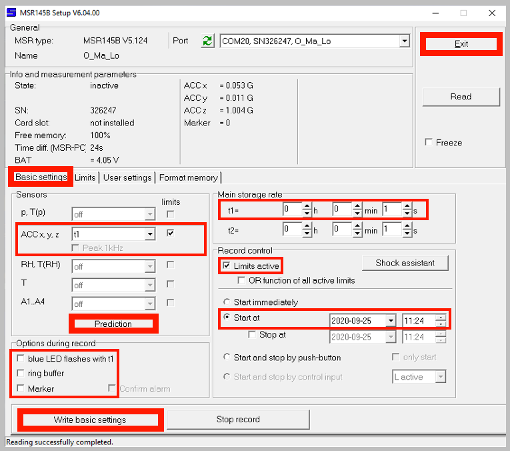
\includegraphics[width=0.7\textwidth,height=\textheight]{chapters/figs/MSRStep5.png}

}

\end{figure}

\hypertarget{hoboware}{%
\section{HOBOware}\label{hoboware}}

The Pendant G Data Logger comes with the free
\href{https://www.onsetcomp.com/hoboware-free-download/}{HOBOware}
software to configure the logger. HOBOware is compatible with Windows
and macOS operating systems. To configure the HOBO Pendant:

\begin{enumerate}
\def\labelenumi{\arabic{enumi}.}
\tightlist
\item
  Download and install the free
  \href{https://www.onsetcomp.com/hoboware-free-download/}{HOBOware}
  software
\item
  Connect a logger to a computer via the HOBO Optic USB Base Station
\item
  Open the HOBOware software
\item
  You can set a name for the logger under \texttt{Name}
\item
  In the \texttt{Sensors} tab and in the
  \texttt{Configure\ Sensors\ to\ Log} section, check the
  \texttt{X-Axis\ Acceleration\ (+/-\ 3g)} box
\item
  From the \texttt{Deployments} tab, set the \texttt{Logging\ Interval}
  to the desired sampling length using the drop-down menu.

  \begin{itemize}
  \tightlist
  \item
    The Mini Buoy has been calibrated to accept sampling rates between 1
    and 10 minutes. Refer to Table~\ref{tbl-1} for sampling duration.
  \end{itemize}
\item
  In the \texttt{Deployments} tab, set the \texttt{Start\ Logging} date
  and time for shortly after your planned deployment\\
\item
  Click \texttt{Delayed\ Start} and disconnect the Pendant logger from
  the computer.
\end{enumerate}

\begin{figure}

{\centering 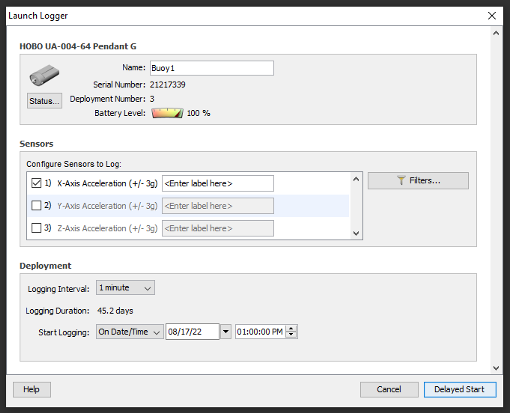
\includegraphics[width=0.7\textwidth,height=\textheight]{chapters/figs/HOBOStep1.png}

}

\end{figure}

\bookmarksetup{startatroot}

\hypertarget{deployment}{%
\chapter{Deployment}\label{deployment}}

Once the Mini Buoy has been assembled and the accelerometer is active,
it is ready deployed at the survey location.

\hypertarget{installing-the-mini-buoy}{%
\section{Installing the Mini Buoy}\label{installing-the-mini-buoy}}

Mini Buoys can be used in single deployments to assess inundation
characteristics at a given location, used in comparative deployments
such as when comparing conditions between restoration and reference
`natural' sites, or used in multi-deployments to gather detailed
hydrodynamic information.

Deployments should last more than 15 days to cover spring and neap tide
variability. When deploying the Mini Buoy in the field, it is important
to consider characteristics of the site and duration of the deployment.
High-energy locations may be subject to excessive scouring that stress
the Mini Buoy tether and may dislodge the anchor. At low-energy
locations excessive sedimentation can bury the Mini Buoy. Using a cable
tie to attach the Mini Buoy tether to an anchor buried \textgreater{}
0.5 m into the ground is recommended for a standard set-up. Gather the
following equipment:

\begin{itemize}
\tightlist
\item
  Large cable tie
\item
  0.7 m length of metal rod with perforations
\end{itemize}

To install the Mini Buoy:

\begin{enumerate}
\def\labelenumi{\arabic{enumi}.}
\tightlist
\item
  Hammer the metal rod into the ground until 1 cm is protruding from the
  surface
\item
  Attach the end of the fishing line chain to the anchor using the cable
  tie
\item
  Move the Mini Buoy 360° around the anchor, and remove any obstructing
  objects
\end{enumerate}

\begin{figure}

{\centering 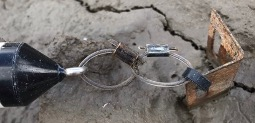
\includegraphics[width=0.7\textwidth,height=\textheight]{chapters/figs/MiniBuoyDeployment.jpg}

}

\end{figure}

\bookmarksetup{startatroot}

\hypertarget{sec-export}{%
\chapter{Export}\label{sec-export}}

After a deployment, the data can be retrieved from the logger and
exported as a .csv data table. It is important to save your data in the
data format that can be recognised by the Mini Buoy App.

\hypertarget{msr145-1}{%
\section{MSR145}\label{msr145-1}}

To export acceleration data from the MSR145 B4 logger:

\begin{enumerate}
\def\labelenumi{\arabic{enumi}.}
\tightlist
\item
  Open the MSR software and double-click \texttt{Csv}
\end{enumerate}

\begin{figure}

{\centering 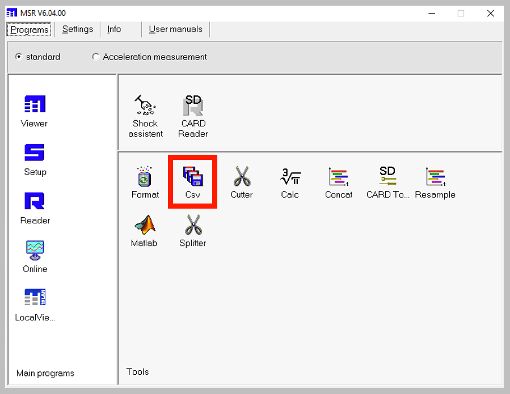
\includegraphics[width=0.7\textwidth,height=\textheight]{chapters/figs/MSRExportStep1.png}

}

\end{figure}

\begin{enumerate}
\def\labelenumi{\arabic{enumi}.}
\setcounter{enumi}{1}
\tightlist
\item
  Choose the settings according to the template below and click
  \texttt{Save}
\end{enumerate}

\begin{figure}

{\centering 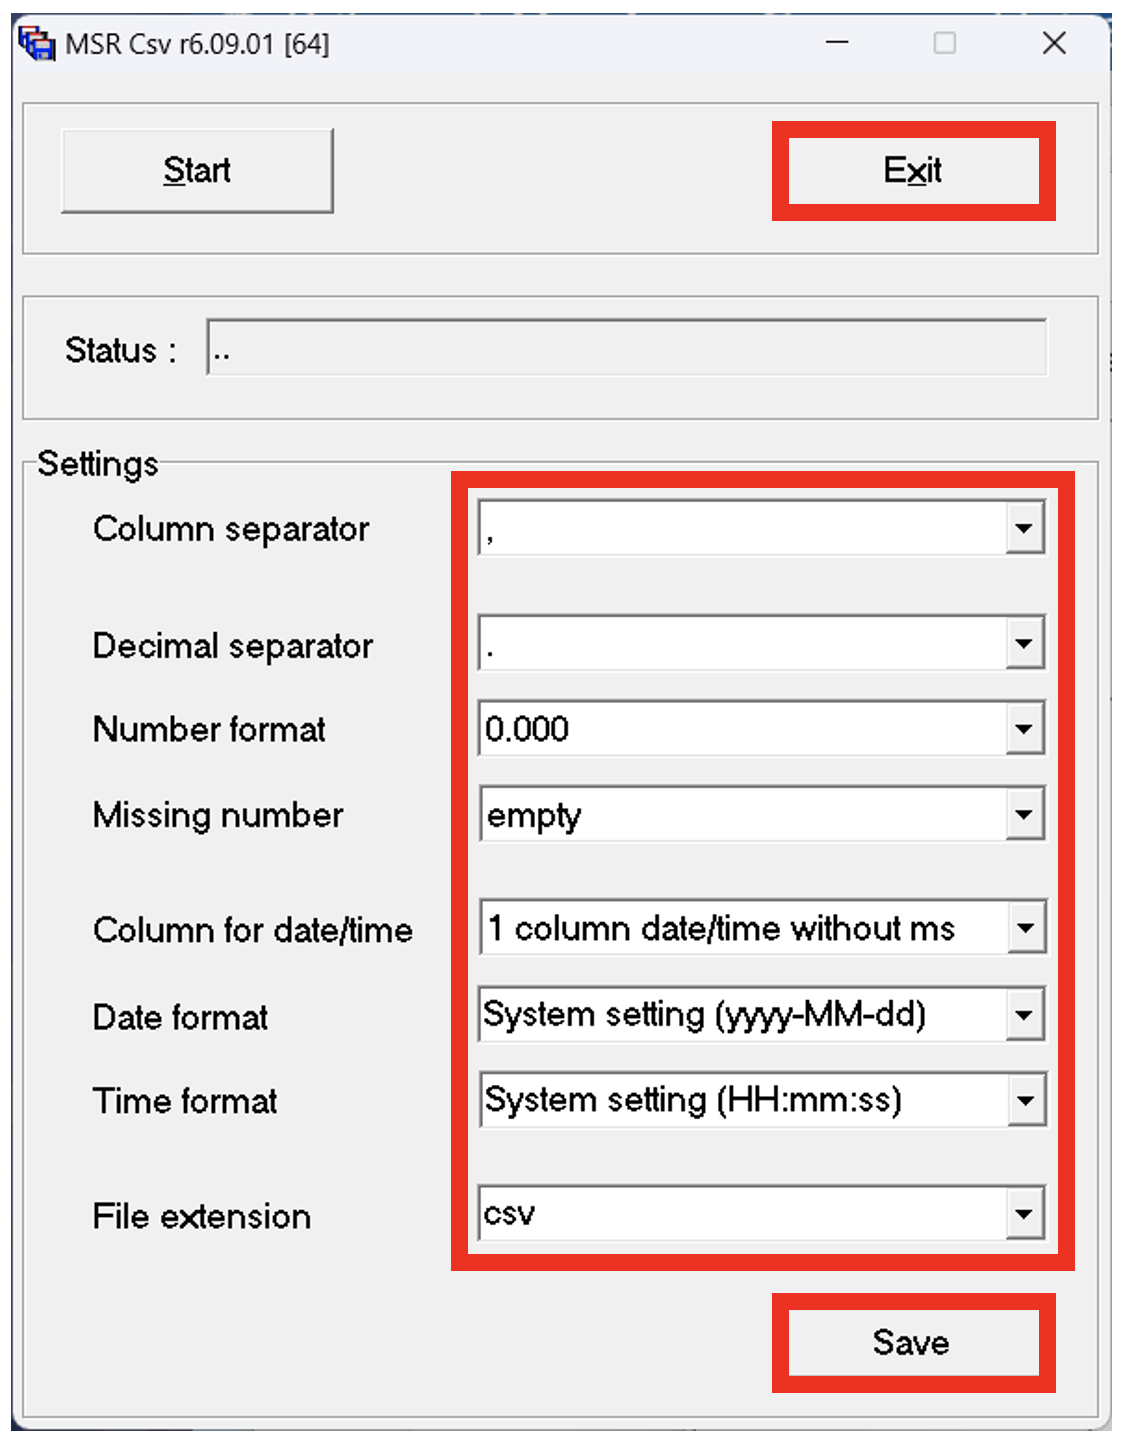
\includegraphics[width=0.7\textwidth,height=\textheight]{chapters/figs/MSRExportStep2.png}

}

\end{figure}

\begin{enumerate}
\def\labelenumi{\arabic{enumi}.}
\setcounter{enumi}{2}
\tightlist
\item
  Connect your data logger with the USB cable
\item
  Open the MSR software and double-click \texttt{Reader}

  \begin{itemize}
  \tightlist
  \item
    The data will be saved onto the computer as an .msr file unique to
    the software
  \end{itemize}
\end{enumerate}

\begin{figure}

{\centering 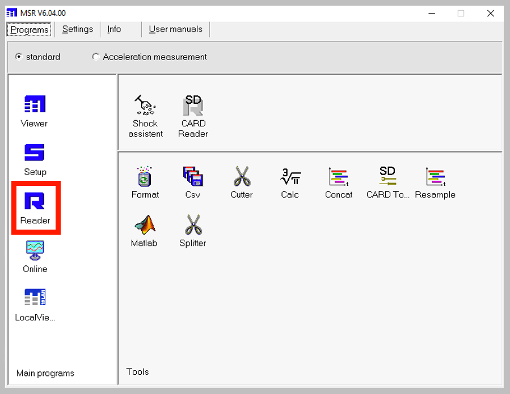
\includegraphics[width=0.7\textwidth,height=\textheight]{chapters/figs/MSRExportStep3.png}

}

\end{figure}

\begin{enumerate}
\def\labelenumi{\arabic{enumi}.}
\setcounter{enumi}{4}
\tightlist
\item
  The MSR software should automatically open the .msr file in order to
  view the data. If nothing happens, double-click \texttt{Viewer} and
  select \texttt{File}, \texttt{Open}, and select the .msr file
\item
  The data should look similar to the graph below, with low tide
  recorded as 0 and high tide recorded around -1. Any data at the start
  and end of the deployment which is not part of the desired measurement
  period can be removed by using the cross arrows button and selecting
  the period of interest. The graph should always start and end with a
  period of low tide (i.e.~0 y acceleration)
\end{enumerate}

\begin{figure}

{\centering 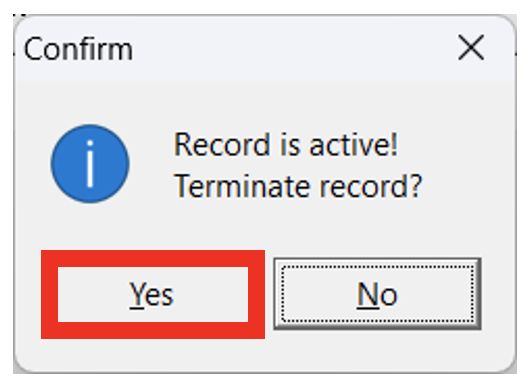
\includegraphics[width=0.7\textwidth,height=\textheight]{chapters/figs/MSRExportStep4.png}

}

\end{figure}

\begin{enumerate}
\def\labelenumi{\arabic{enumi}.}
\setcounter{enumi}{6}
\tightlist
\item
  Select \texttt{File}, \texttt{Export\ time\ window\ as\ text…}, and
  select an appropriate folder to save the data as a .csv file
\end{enumerate}

\begin{figure}

{\centering 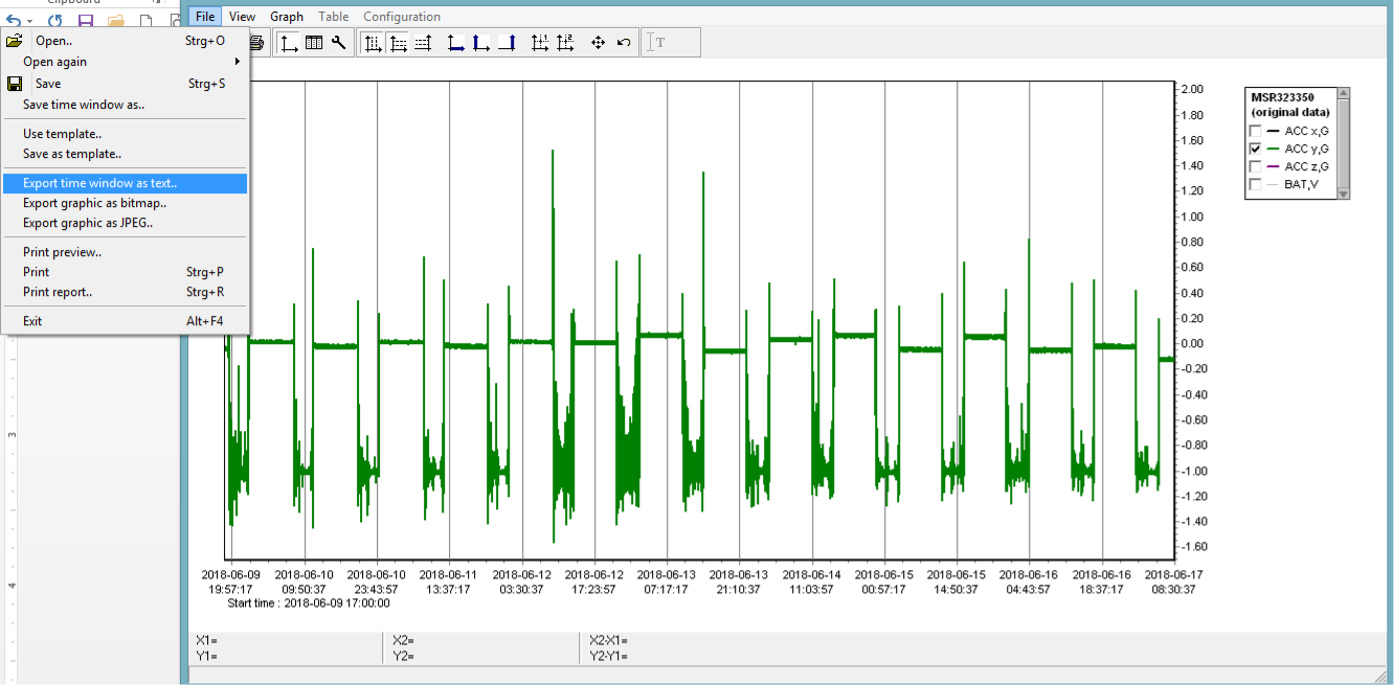
\includegraphics[width=0.7\textwidth,height=\textheight]{chapters/figs/MSRExportStep5.png}

}

\end{figure}

\hypertarget{hoboware-1}{%
\section{HOBOware}\label{hoboware-1}}

To export acceleration data from the Pendant G Data Logger:

\begin{enumerate}
\def\labelenumi{\arabic{enumi}.}
\tightlist
\item
  Open the HOBOware software
\item
  Open the preferences window by selecting \texttt{HOBOware} and
  \texttt{Preferences...}
\end{enumerate}

\begin{figure}

{\centering 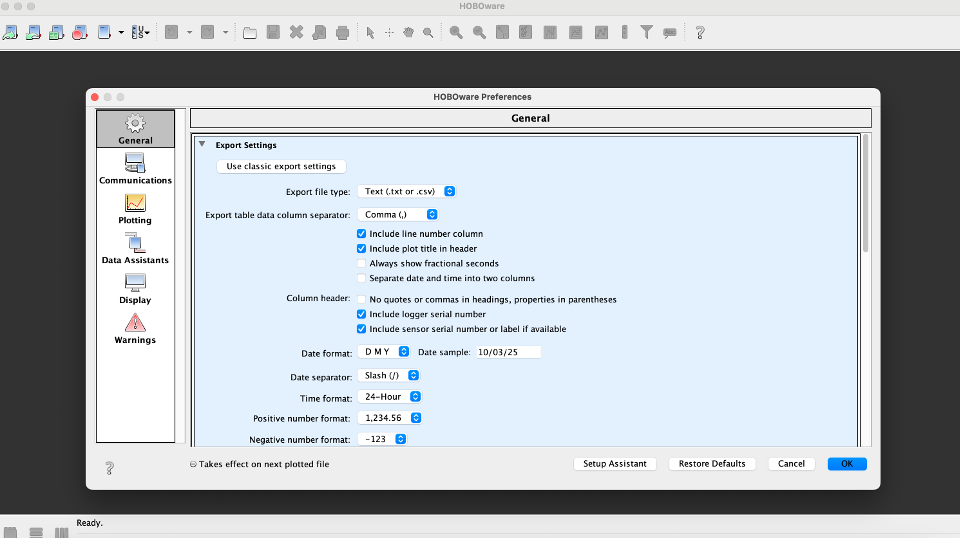
\includegraphics[width=0.7\textwidth,height=\textheight]{chapters/figs/HOBOExportStep1.png}

}

\end{figure}

\begin{enumerate}
\def\labelenumi{\arabic{enumi}.}
\setcounter{enumi}{2}
\tightlist
\item
  Select \texttt{General}, \texttt{Export\ Settings}, and ensure that
  \texttt{Separate\ date\ and\ time\ into\ two\ columns} is unchecked
\item
  Press \texttt{OK}
\end{enumerate}

\begin{figure}

{\centering 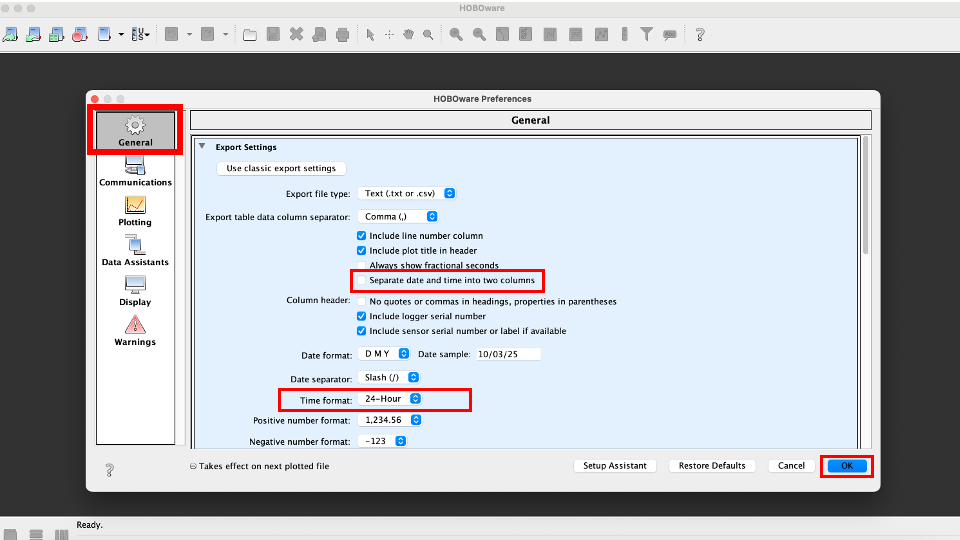
\includegraphics[width=0.7\textwidth,height=\textheight]{chapters/figs/HOBOExportStep2.png}

}

\end{figure}

\begin{enumerate}
\def\labelenumi{\arabic{enumi}.}
\setcounter{enumi}{4}
\tightlist
\item
  Select \texttt{Plot\ Setup}
\item
  Check the \texttt{X\ Accel} box
\end{enumerate}

\begin{figure}

{\centering 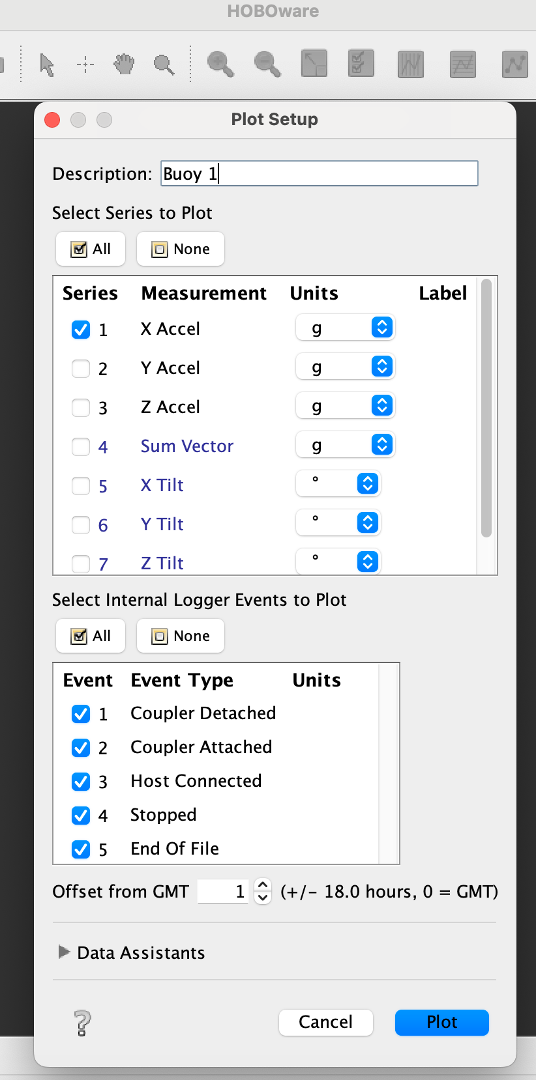
\includegraphics{chapters/figs/HOBOExportStep3.png}

}

\end{figure}

\begin{enumerate}
\def\labelenumi{\arabic{enumi}.}
\setcounter{enumi}{6}
\tightlist
\item
  Select \texttt{Plot}
\item
  Select \texttt{Export}
\item
  Save the file as \texttt{.csv}
\end{enumerate}

\begin{figure}

{\centering 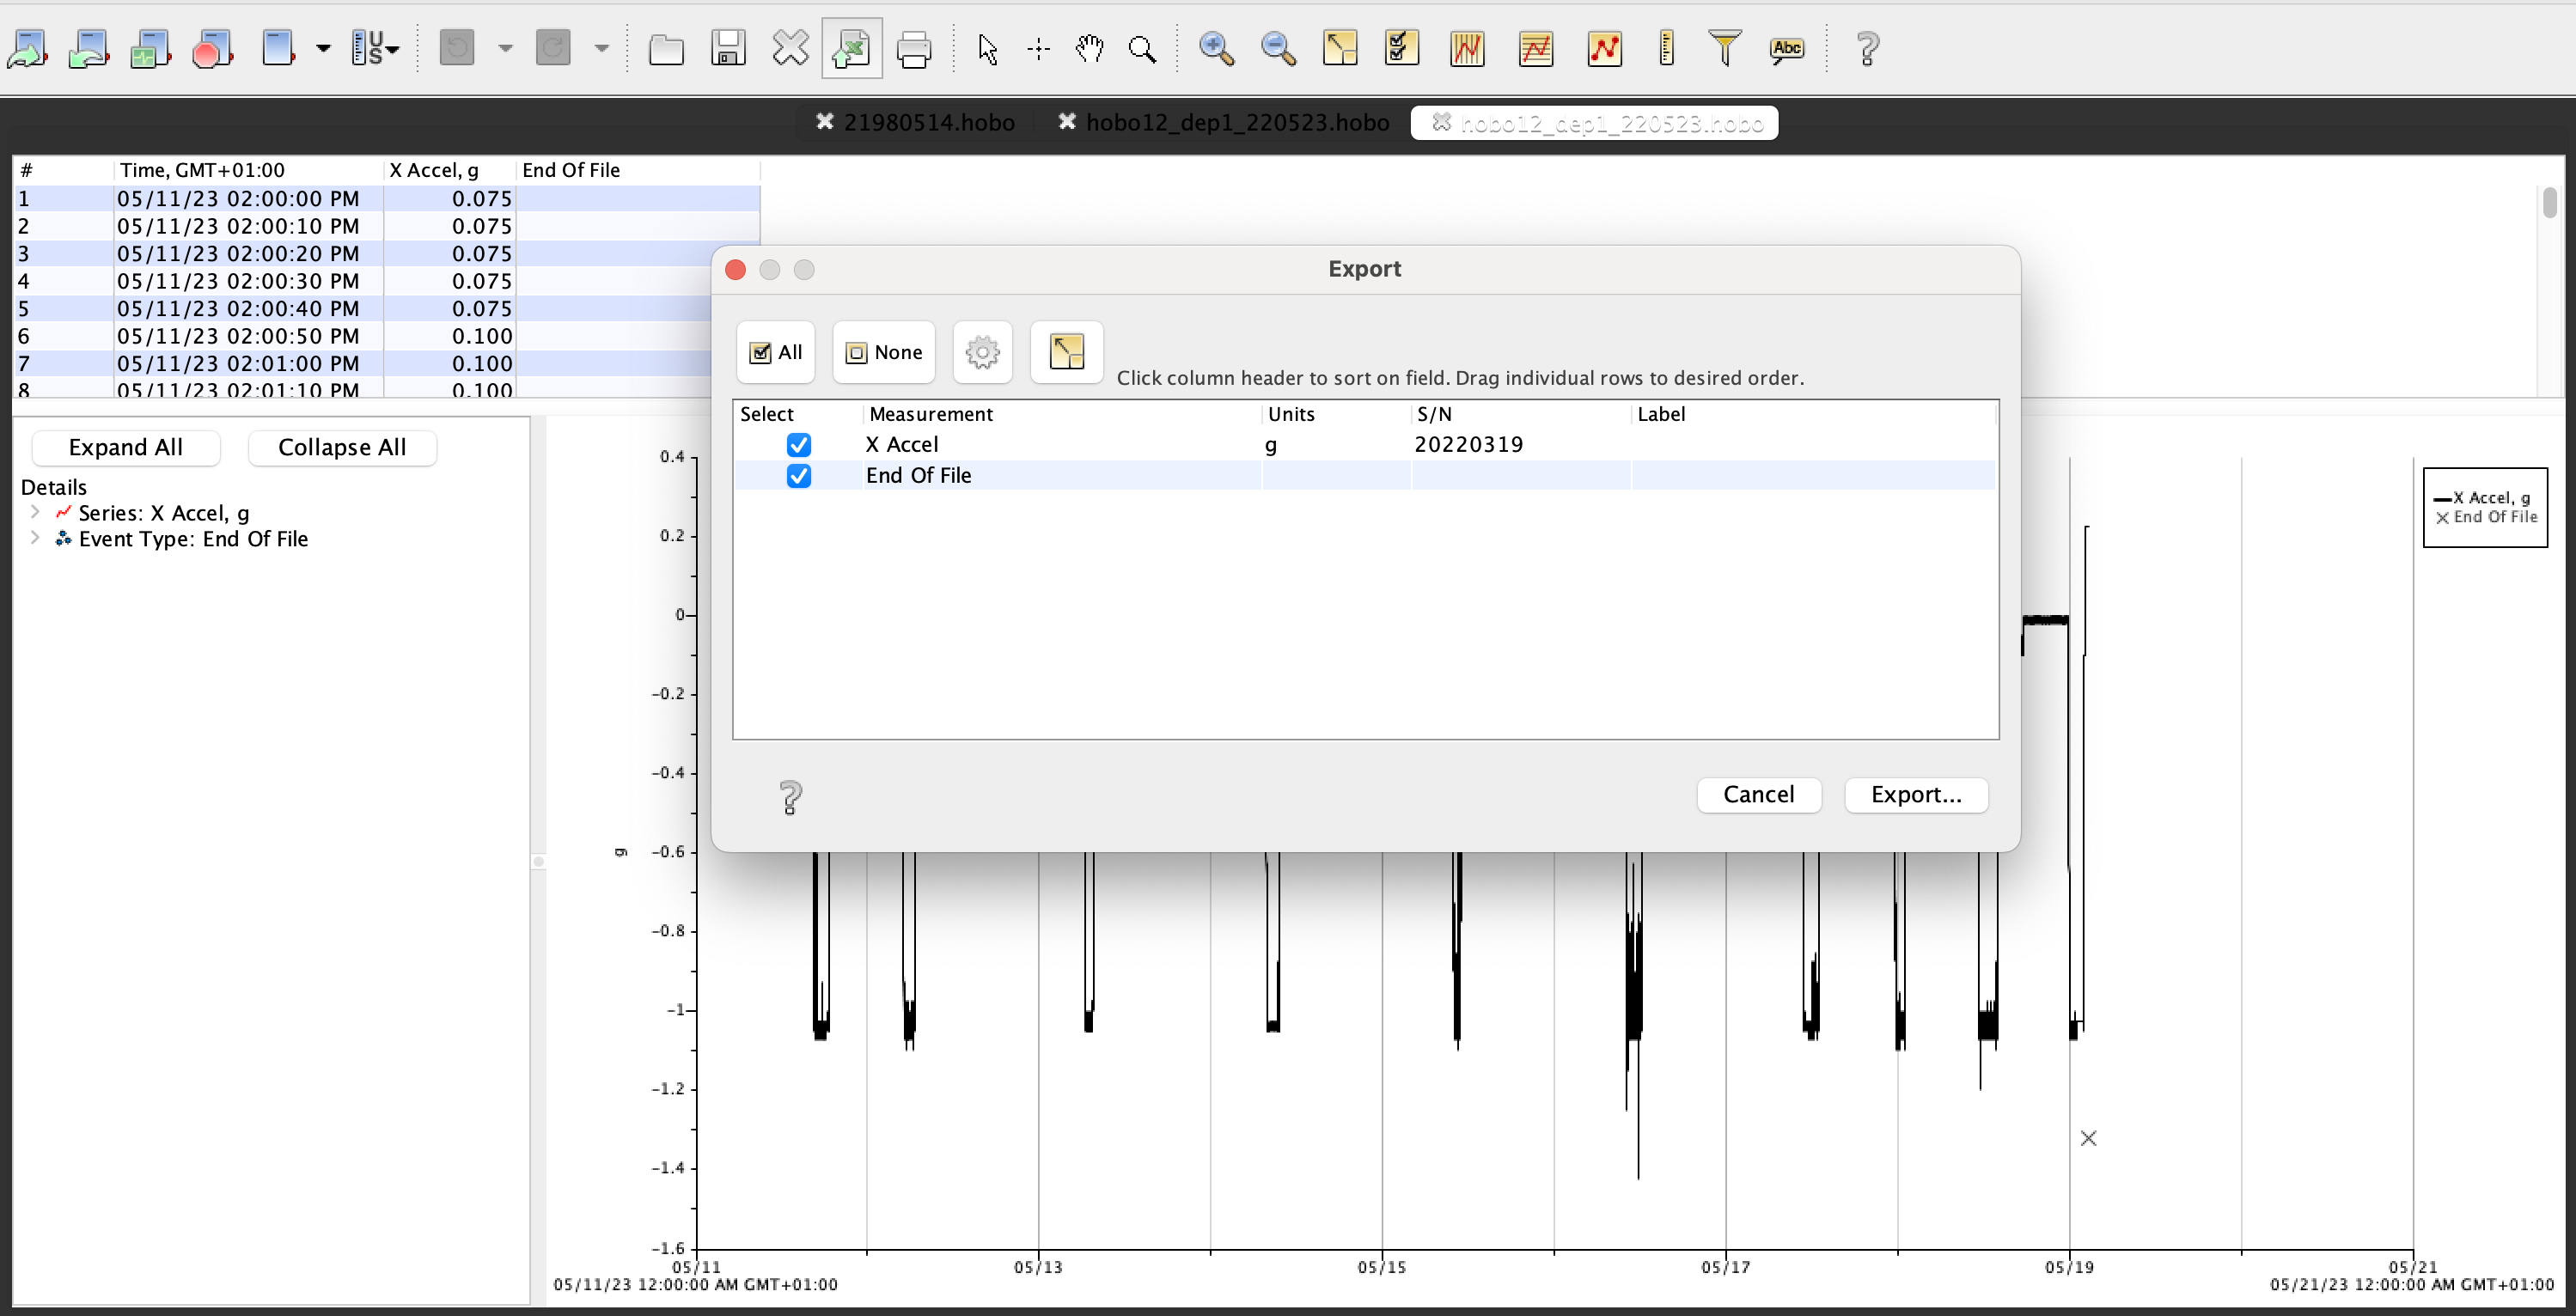
\includegraphics[width=0.7\textwidth,height=\textheight]{chapters/figs/HOBOExportStep4.png}

}

\end{figure}

\bookmarksetup{startatroot}

\hypertarget{analysis}{%
\chapter{Analysis}\label{analysis}}

The Mini Buoy App is an open-source tool for reading and interpreting
data gathered by any of the three Mini Buoy designs.

\begin{figure}

{\centering 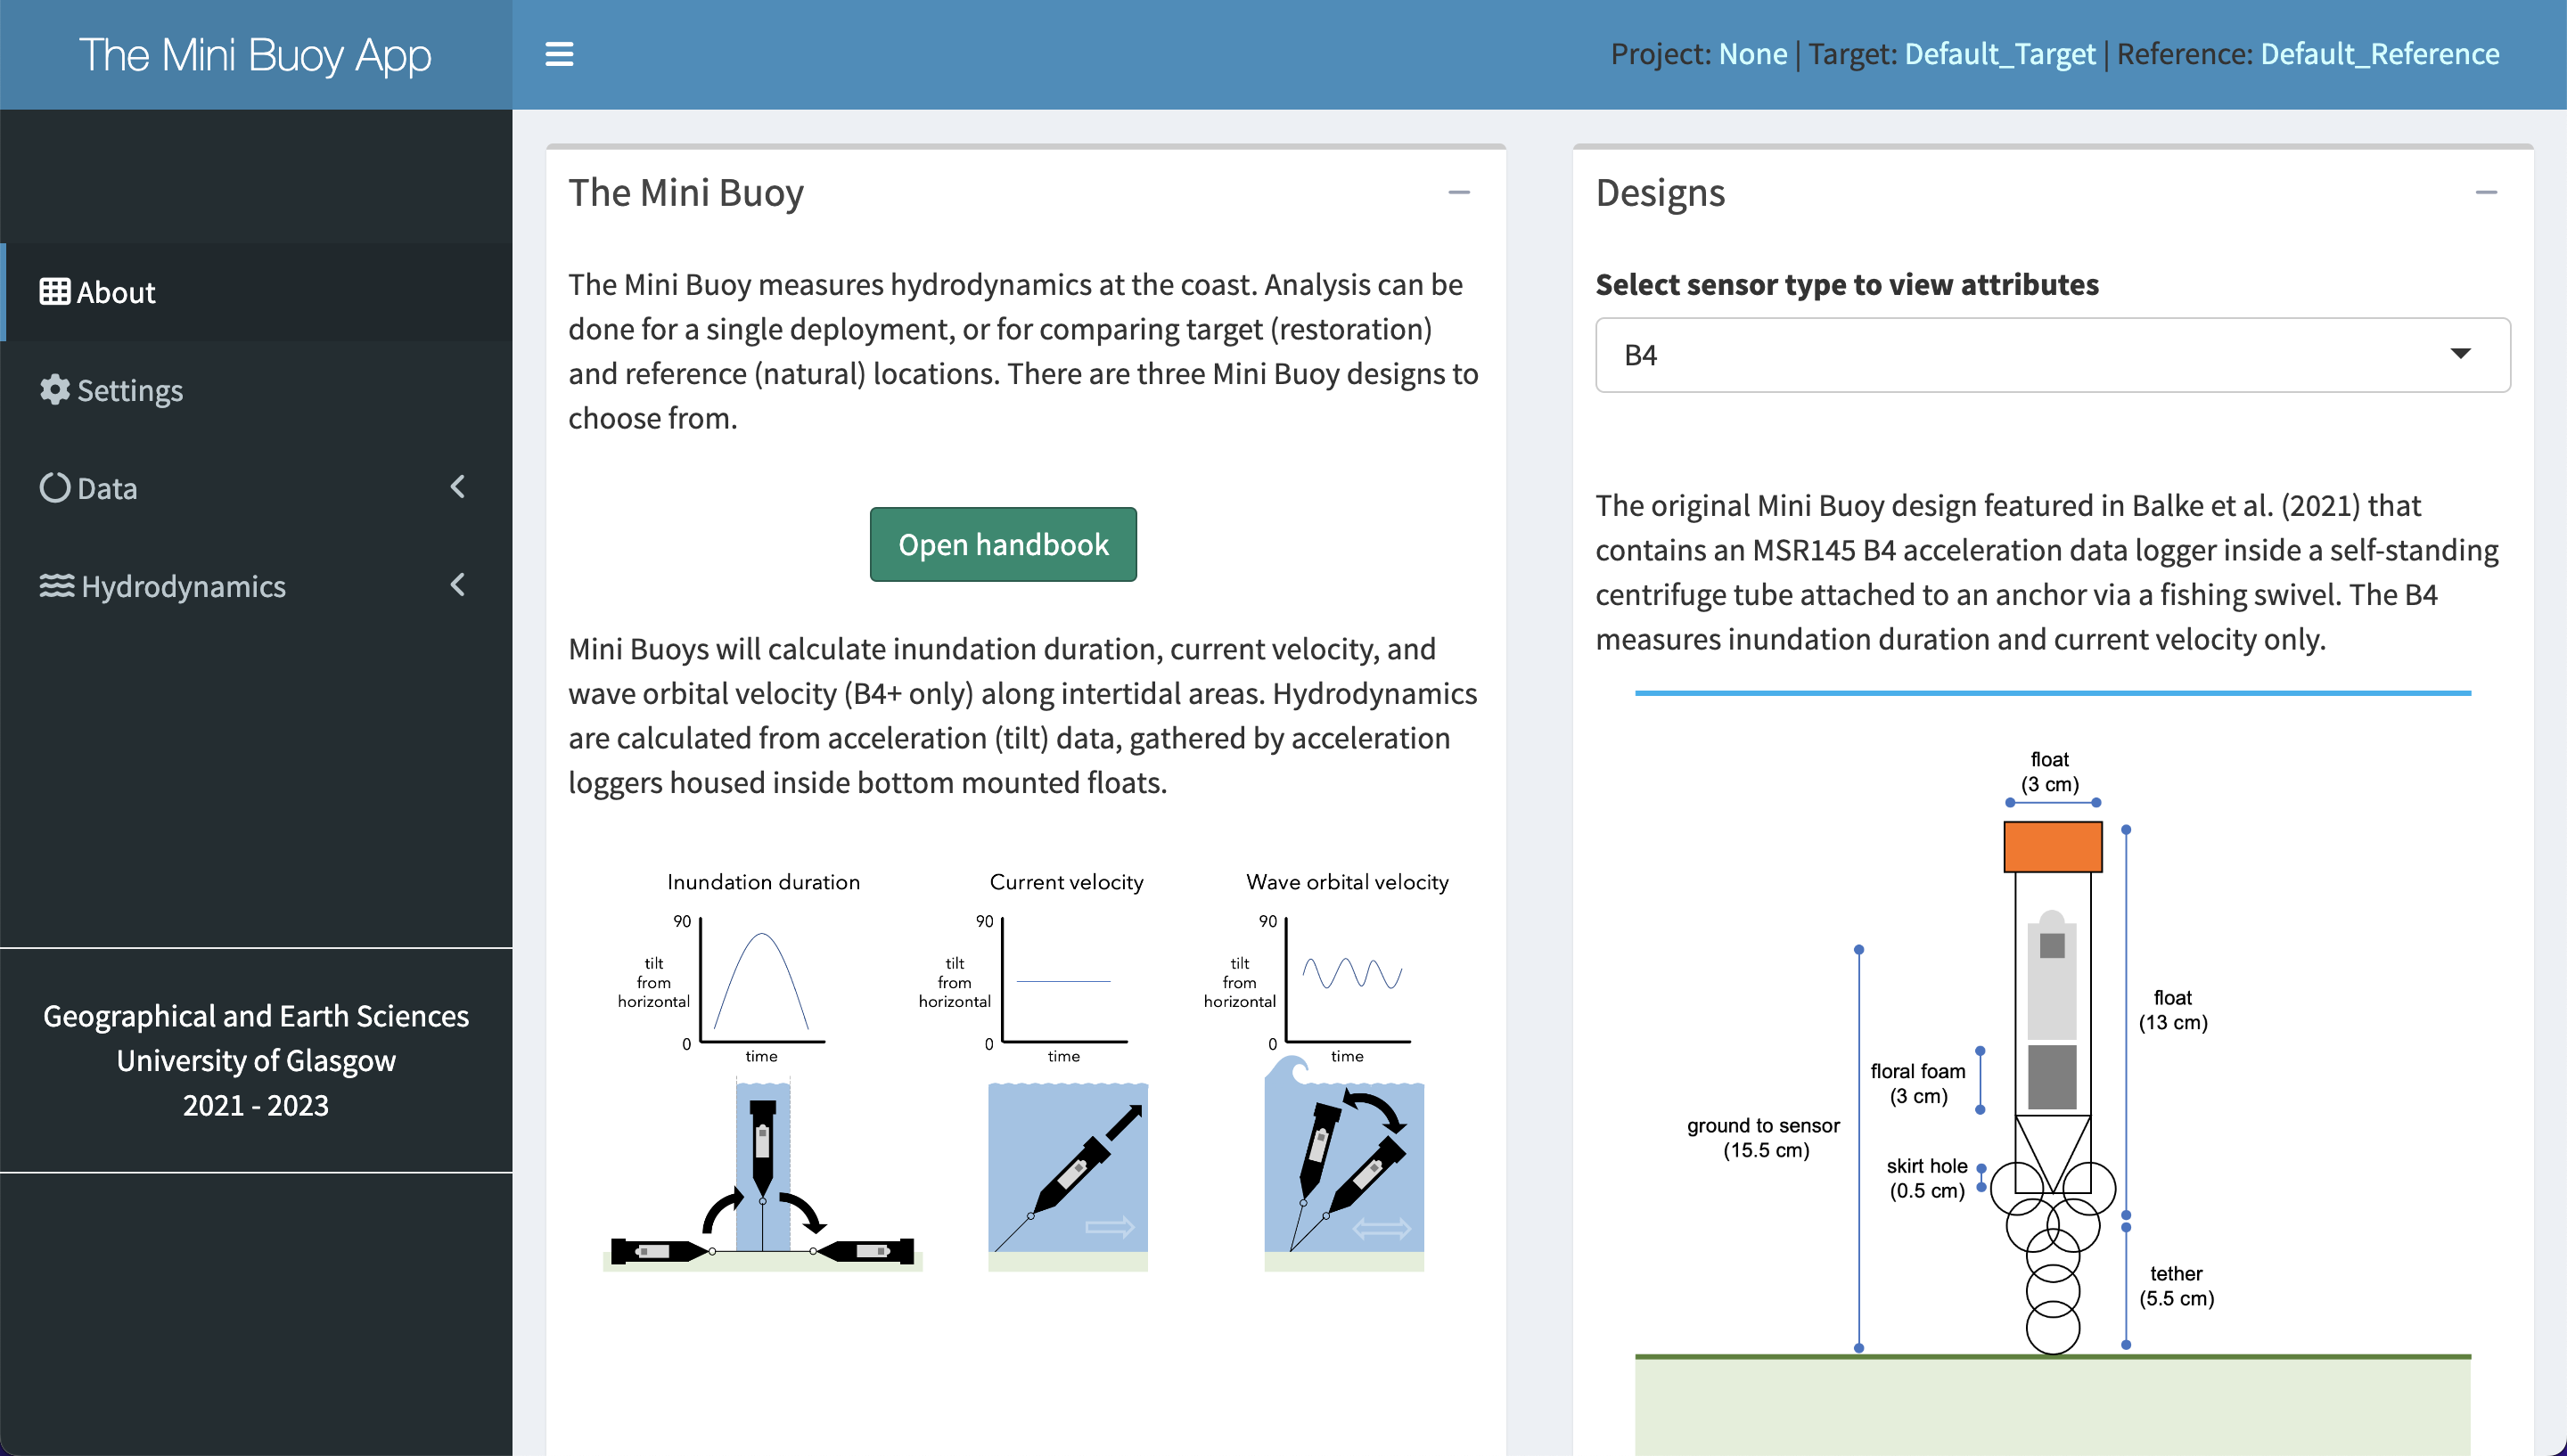
\includegraphics[width=1\textwidth,height=\textheight]{chapters/figs/About.png}

}

\end{figure}

\hypertarget{installation}{%
\section{Installation}\label{installation}}

The Mini Buoy App is a Shiny application. The App can either be executed
as a standalone App (Windows PC only) or directly through RStudio (all
systems).

\hypertarget{standalone-application}{%
\subsection{Standalone Application}\label{standalone-application}}

\begin{enumerate}
\def\labelenumi{\arabic{enumi}.}
\tightlist
\item
  Download the App
  \href{https://cloudstore.zih.tu-dresden.de/index.php/s/7ES7xq2tzMBfNm5}{here.}
\item
  Unzip the folder to a desired location on your system.
\item
  Double-click on the \texttt{MiniBuoyApp.bat} file to launch the App.
\end{enumerate}

\begin{tcolorbox}[enhanced jigsaw, bottomrule=.15mm, leftrule=.75mm, bottomtitle=1mm, breakable, opacityback=0, colback=white, left=2mm, toprule=.15mm, opacitybacktitle=0.6, arc=.35mm, colframe=quarto-callout-note-color-frame, toptitle=1mm, titlerule=0mm, colbacktitle=quarto-callout-note-color!10!white, coltitle=black, title=\textcolor{quarto-callout-note-color}{\faInfo}\hspace{0.5em}{Note}, rightrule=.15mm]

The App is currently only compatible with Windows PC. Mac users should
run the App directly via RStudio (see below).

\end{tcolorbox}

\hypertarget{running-within-rstudio}{%
\subsection{Running within RStudio}\label{running-within-rstudio}}

\begin{enumerate}
\def\labelenumi{\arabic{enumi}.}
\tightlist
\item
  Install R and RStudio
  \href{https://posit.co/download/rstudio-desktop/}{here.}
\item
  Launch the App via GitHub, and install the \texttt{shiny} package if
  necessary:
\end{enumerate}

\begin{Shaded}
\begin{Highlighting}[]
\ControlFlowTok{if}\NormalTok{(}\SpecialCharTok{!}\FunctionTok{require}\NormalTok{(}\StringTok{\textquotesingle{}shiny\textquotesingle{}}\NormalTok{)) }\FunctionTok{install.packages}\NormalTok{(}\StringTok{\textquotesingle{}shiny\textquotesingle{}}\NormalTok{)}
\FunctionTok{runGitHub}\NormalTok{(}\AttributeTok{repo =} \StringTok{\textquotesingle{}MiniBuoy{-}App\textquotesingle{}}\NormalTok{, }\AttributeTok{user =} \StringTok{\textquotesingle{}Ale0430\textquotesingle{}}\NormalTok{, }\AttributeTok{launch.browser =}\NormalTok{ T)}
\end{Highlighting}
\end{Shaded}

\hypertarget{source-code}{%
\subsection{Source code}\label{source-code}}

Users are also able to download the source code of the app from GitHub
repository \href{https://github.com/Ale0430/MiniBuoy-App}{here}.

\hypertarget{using-the-app}{%
\section{Using the App}\label{using-the-app}}

The Mini Buoy App is optimised to contrast hydrodynamic characterstics
of intertidal environments at reference (e.g., estabished mangrove edge)
and target (e.g., earmarked for mangrove planting) sites. As well as
providing a comparison, hydrodynamic conditions of reference and target
sites are reported separately. The App will function if only a single
Mini Buoy dataset is used, albeit no comparison will be available.
Reference and target sites can be used interchangeably.

This tutorial is based on the default reference and target dataset
provided with the App.

\hypertarget{sec-custon}{%
\subsection{Settings}\label{sec-custon}}

Selecting a location to save outputs is optional. If not set, the App
defaults to saving output in the same location that the App is running.

\begin{enumerate}
\def\labelenumi{\arabic{enumi}.}
\tightlist
\item
  Select \texttt{Settings} from the left-hand menu.
\item
  Select \texttt{Browse\ to\ select\ a\ project\ folder}.
\item
  Navigate to a desired location to save output generated by the App.
  Root directories can be accessed by selecting the top-right drop-down
  menu
  (
\includegraphics[width=0.15\textwidth,height=\textheight]{chapters/figs/NavigatorIcon.png}).
  Use the folder structure in the left-hand window to navigate to the
  desired location and click \texttt{Select}.
\item
  Click \texttt{Create\ project}. The working directory will now be
  displayed in the \texttt{Project} window and at the top-right corner
  of the window.
\end{enumerate}

\begin{tcolorbox}[enhanced jigsaw, bottomrule=.15mm, leftrule=.75mm, bottomtitle=1mm, breakable, opacityback=0, colback=white, left=2mm, toprule=.15mm, opacitybacktitle=0.6, arc=.35mm, colframe=quarto-callout-tip-color-frame, toptitle=1mm, titlerule=0mm, colbacktitle=quarto-callout-tip-color!10!white, coltitle=black, title=\textcolor{quarto-callout-tip-color}{\faLightbulb}\hspace{0.5em}{Tip}, rightrule=.15mm]

Formats for exported data (\texttt{.csv} or \texttt{.xlsx}) and figures
(\texttt{.jpg}, \texttt{.pdf}, or \texttt{.rdata}) can be chosen, and
figure title, prefix, and theme can be chosen.

\end{tcolorbox}

\begin{figure}

{\centering 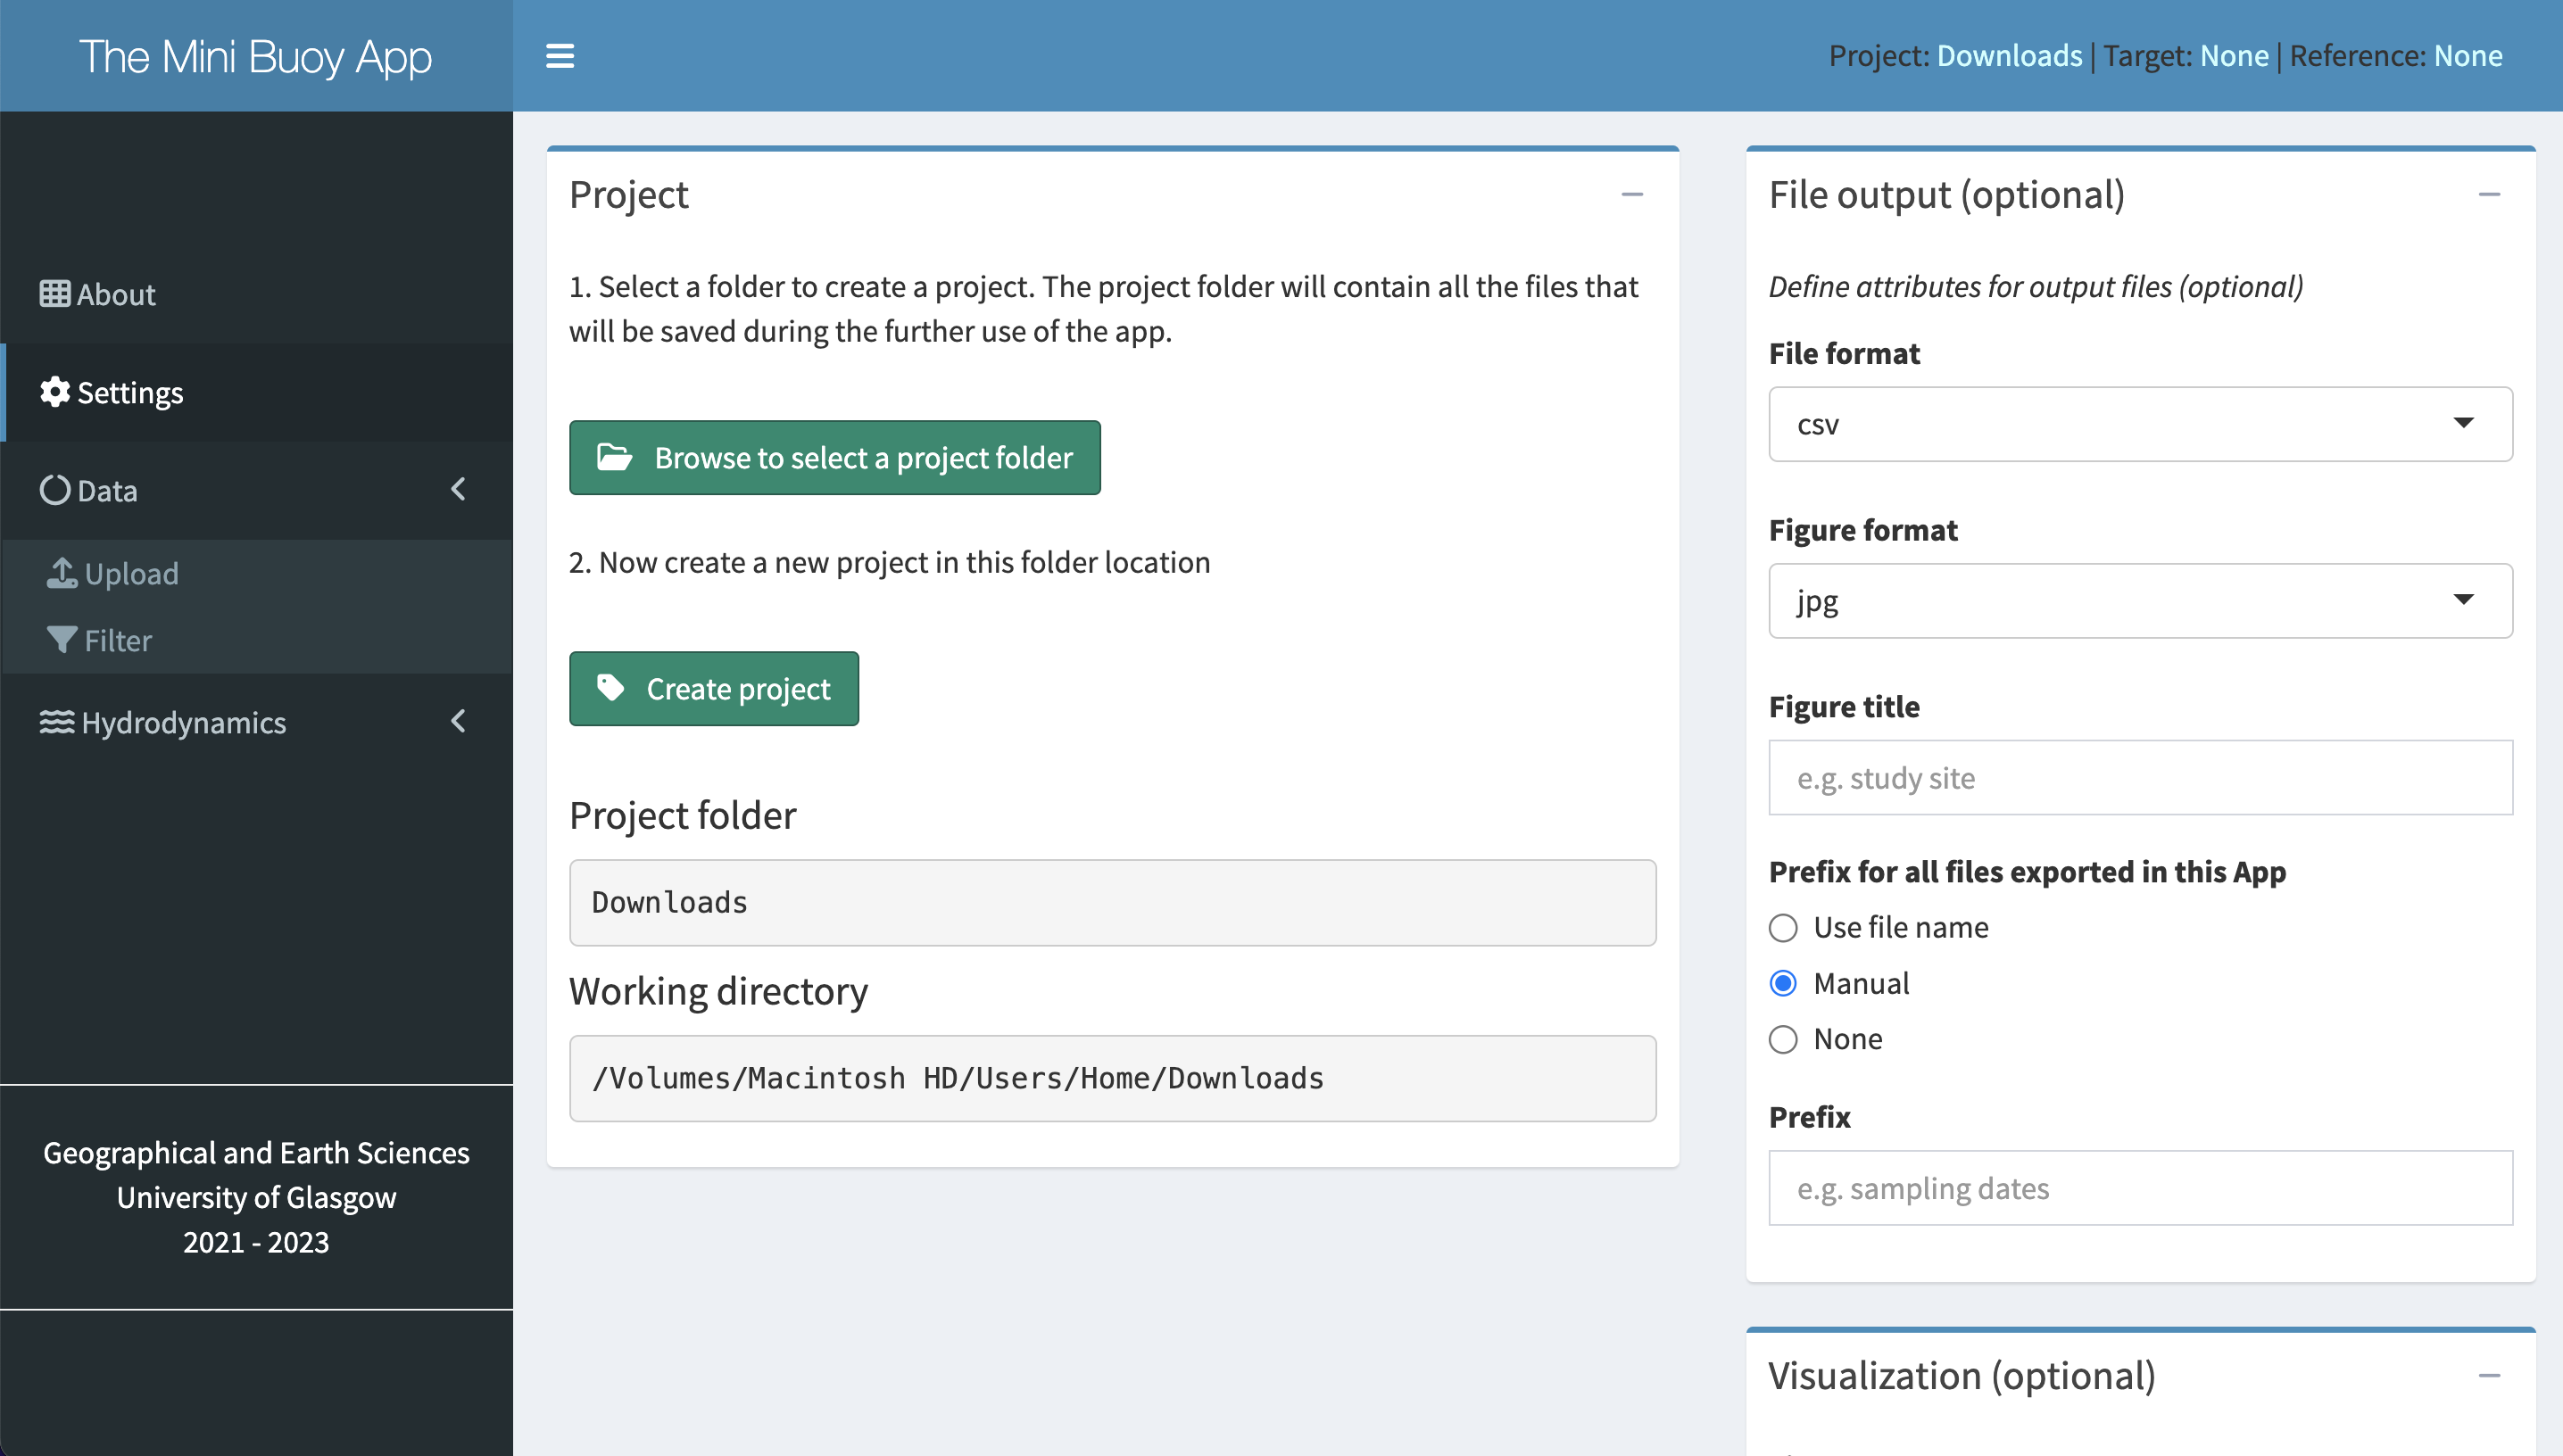
\includegraphics[width=1\textwidth,height=\textheight]{chapters/figs/Settings.png}

}

\end{figure}

\hypertarget{sec-default}{%
\subsection{Upload data}\label{sec-default}}

Users have the option of uploading their own data, or using a default
dataset supplied with the App. Once either is loaded, a summary table
per dataset will be displayed. This table gives the user an initial
quality control option to confirm whether the raw data is as expected
(e.g., are the columns being identified correctly? is the duration of
the survey as expected? is the amount of data as expected according to
the sampling rate?).

\begin{enumerate}
\def\labelenumi{\arabic{enumi}.}
\tightlist
\item
  Select \texttt{Data} and \texttt{Upload} from the left-hand menu.
\item
  Select the Mini Buoy design being used for Target and Reference sites.
  Options for uploading data will then appear.
\item
  Select \texttt{Browse...} and navigate to a desired dataset.
  Alternatively, check the `Use default B4+ data' box(es) to use in the
  analysis.
\item
  Select \texttt{Use\ data}. The file name will appear in the top-right
  corner if uploaded successfully.
\end{enumerate}

\begin{tcolorbox}[enhanced jigsaw, bottomrule=.15mm, leftrule=.75mm, bottomtitle=1mm, breakable, opacityback=0, colback=white, left=2mm, toprule=.15mm, opacitybacktitle=0.6, arc=.35mm, colframe=quarto-callout-important-color-frame, toptitle=1mm, titlerule=0mm, colbacktitle=quarto-callout-important-color!10!white, coltitle=black, title=\textcolor{quarto-callout-important-color}{\faExclamation}\hspace{0.5em}{Important}, rightrule=.15mm]

Please ensure the data has been exported from the Mini Buoy in the
correct format (see Chapter~\ref{sec-export}).

\end{tcolorbox}

\begin{figure}

{\centering 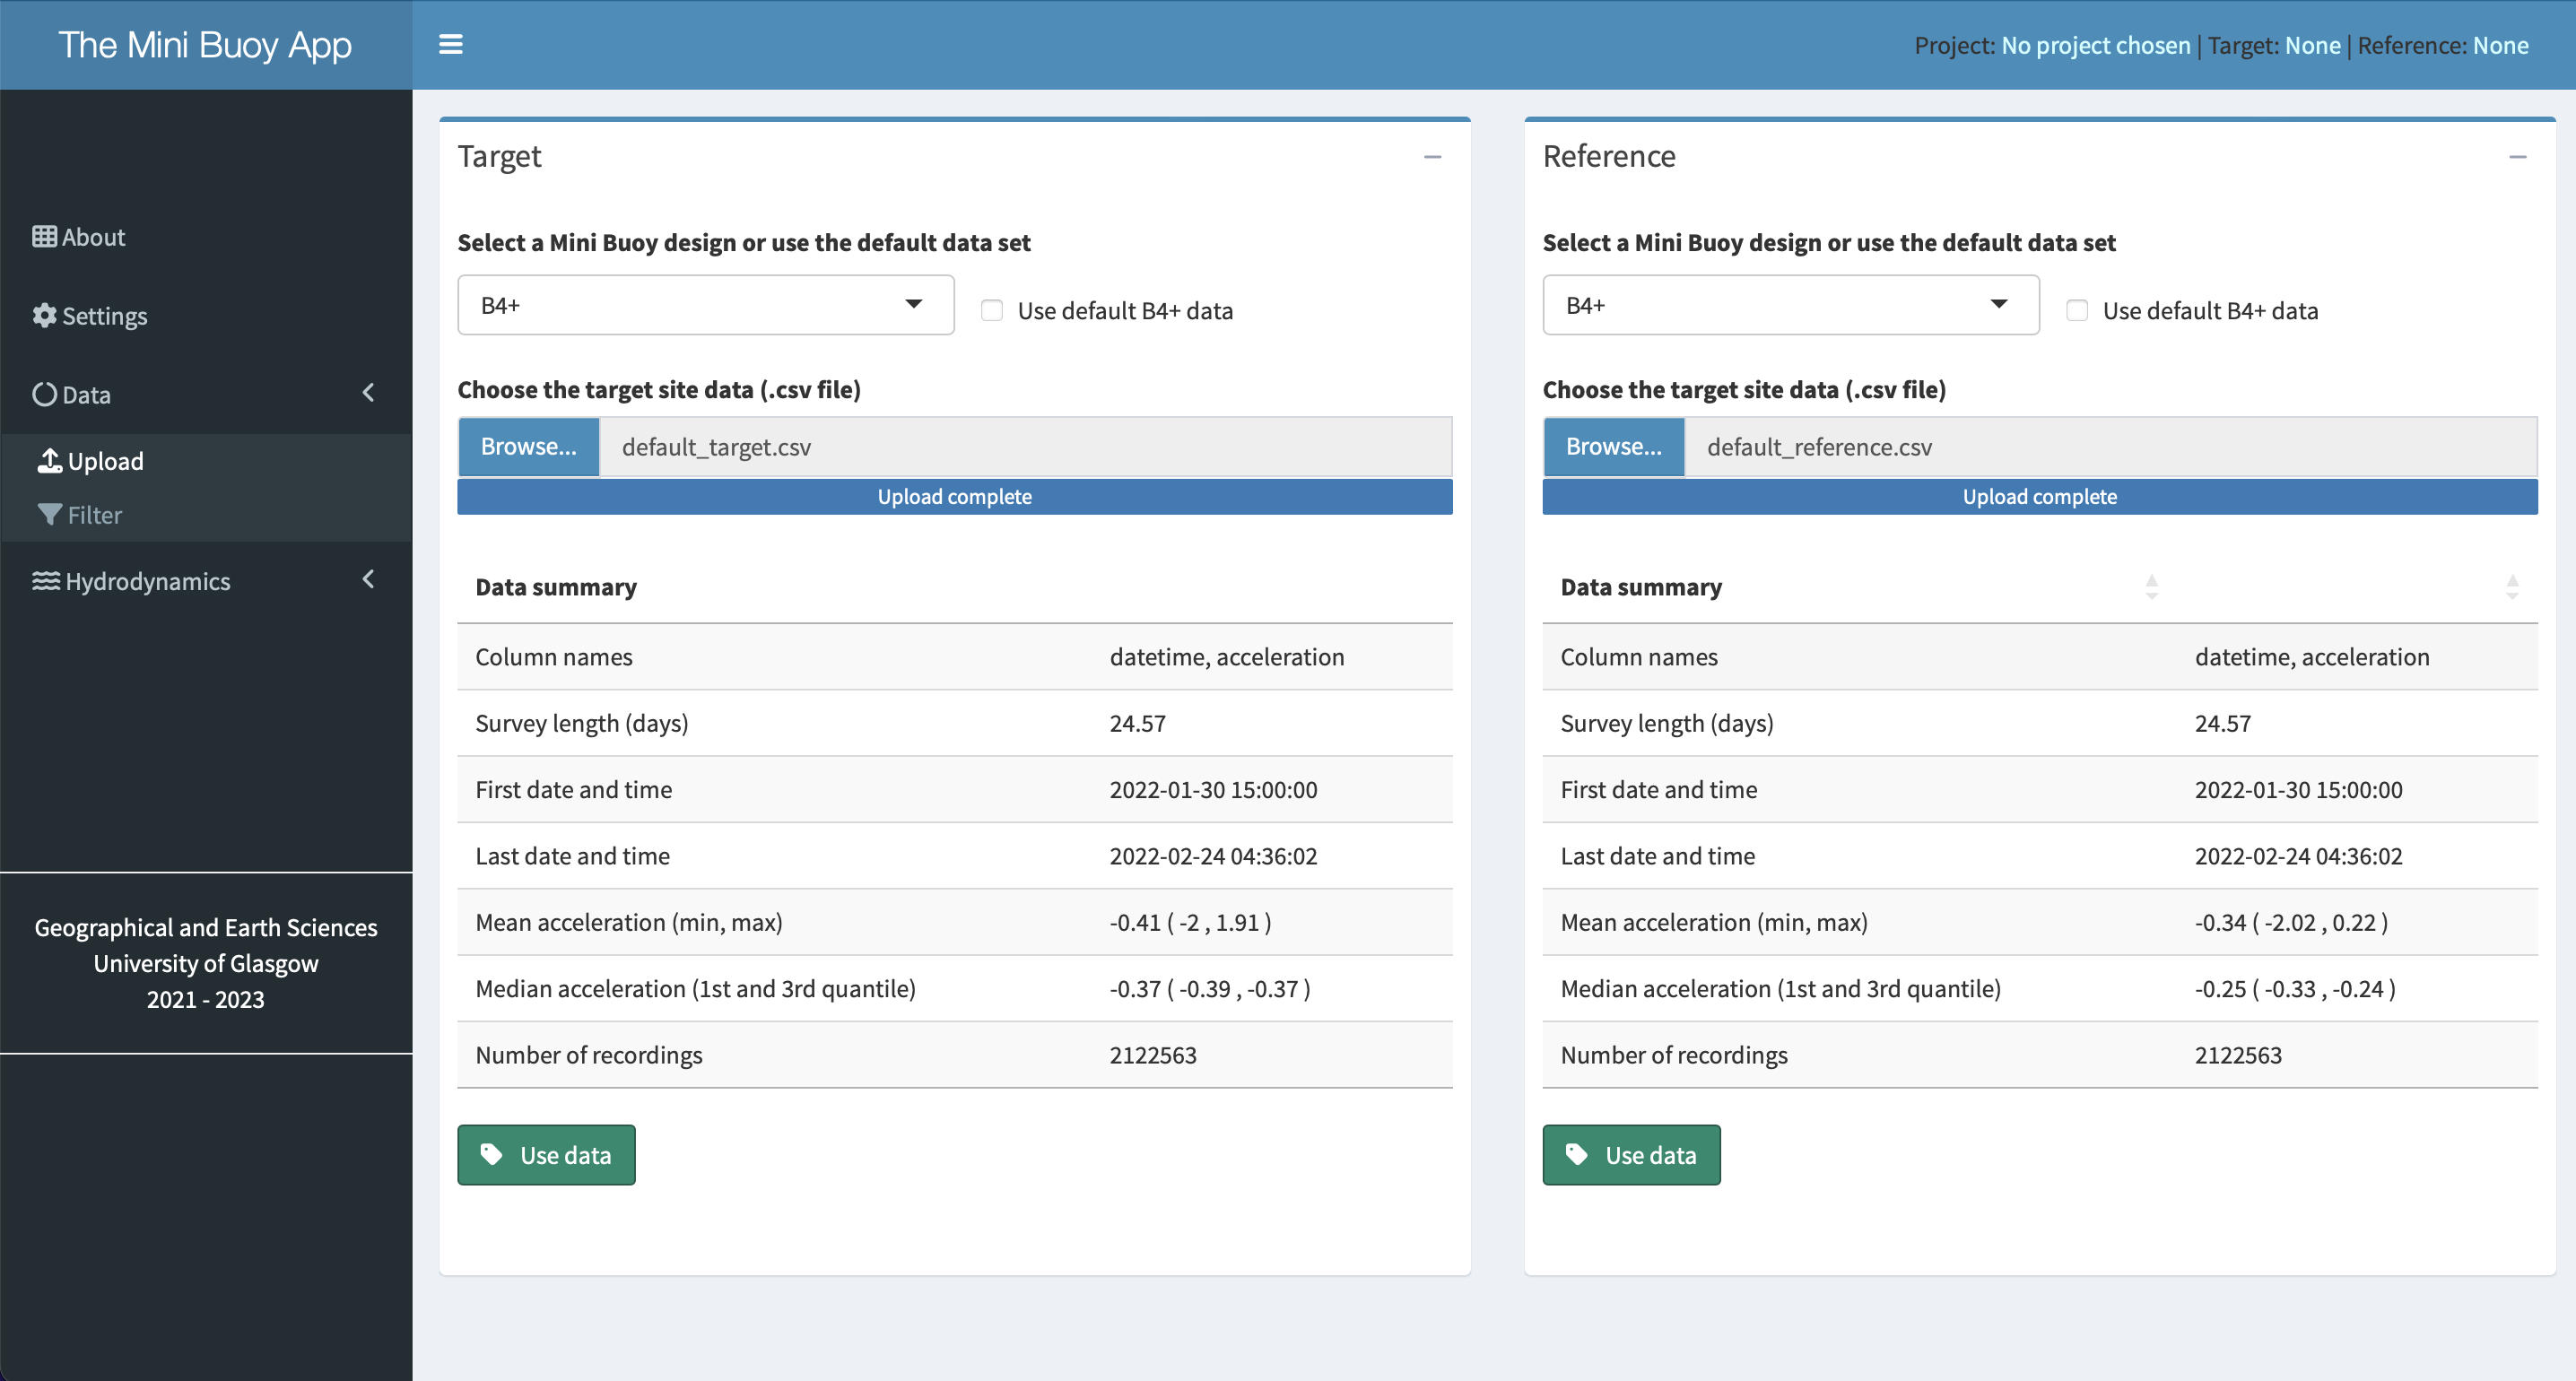
\includegraphics[width=1\textwidth,height=\textheight]{chapters/figs/DataUpload.png}

}

\end{figure}

\hypertarget{filter-data-optional}{%
\subsection{Filter data (optional)}\label{filter-data-optional}}

Users may wish to `clean' the data before analysis to remove any
spurious data (e.g., acceleration values for when the Mini Buoy was in
transit to/from the deployment site). This can be done by filtering
usable data between two datetimes. The raw data can also be plotted to
aid in selecting appropriate start/end times.

\begin{enumerate}
\def\labelenumi{\arabic{enumi}.}
\tightlist
\item
  Select \texttt{Data} and \texttt{Filter} from the left-hand menu.
\item
  Enter the start and end datetimes and select \texttt{Apply\ filter}
  for target and reference datasets as applicable.
\item
  Select \texttt{Render\ figure} to view raw data. The filtered data
  will be displayed. See \textbf{Troubleshooting} to see how the raw
  data should look.
\end{enumerate}

\begin{figure}

{\centering 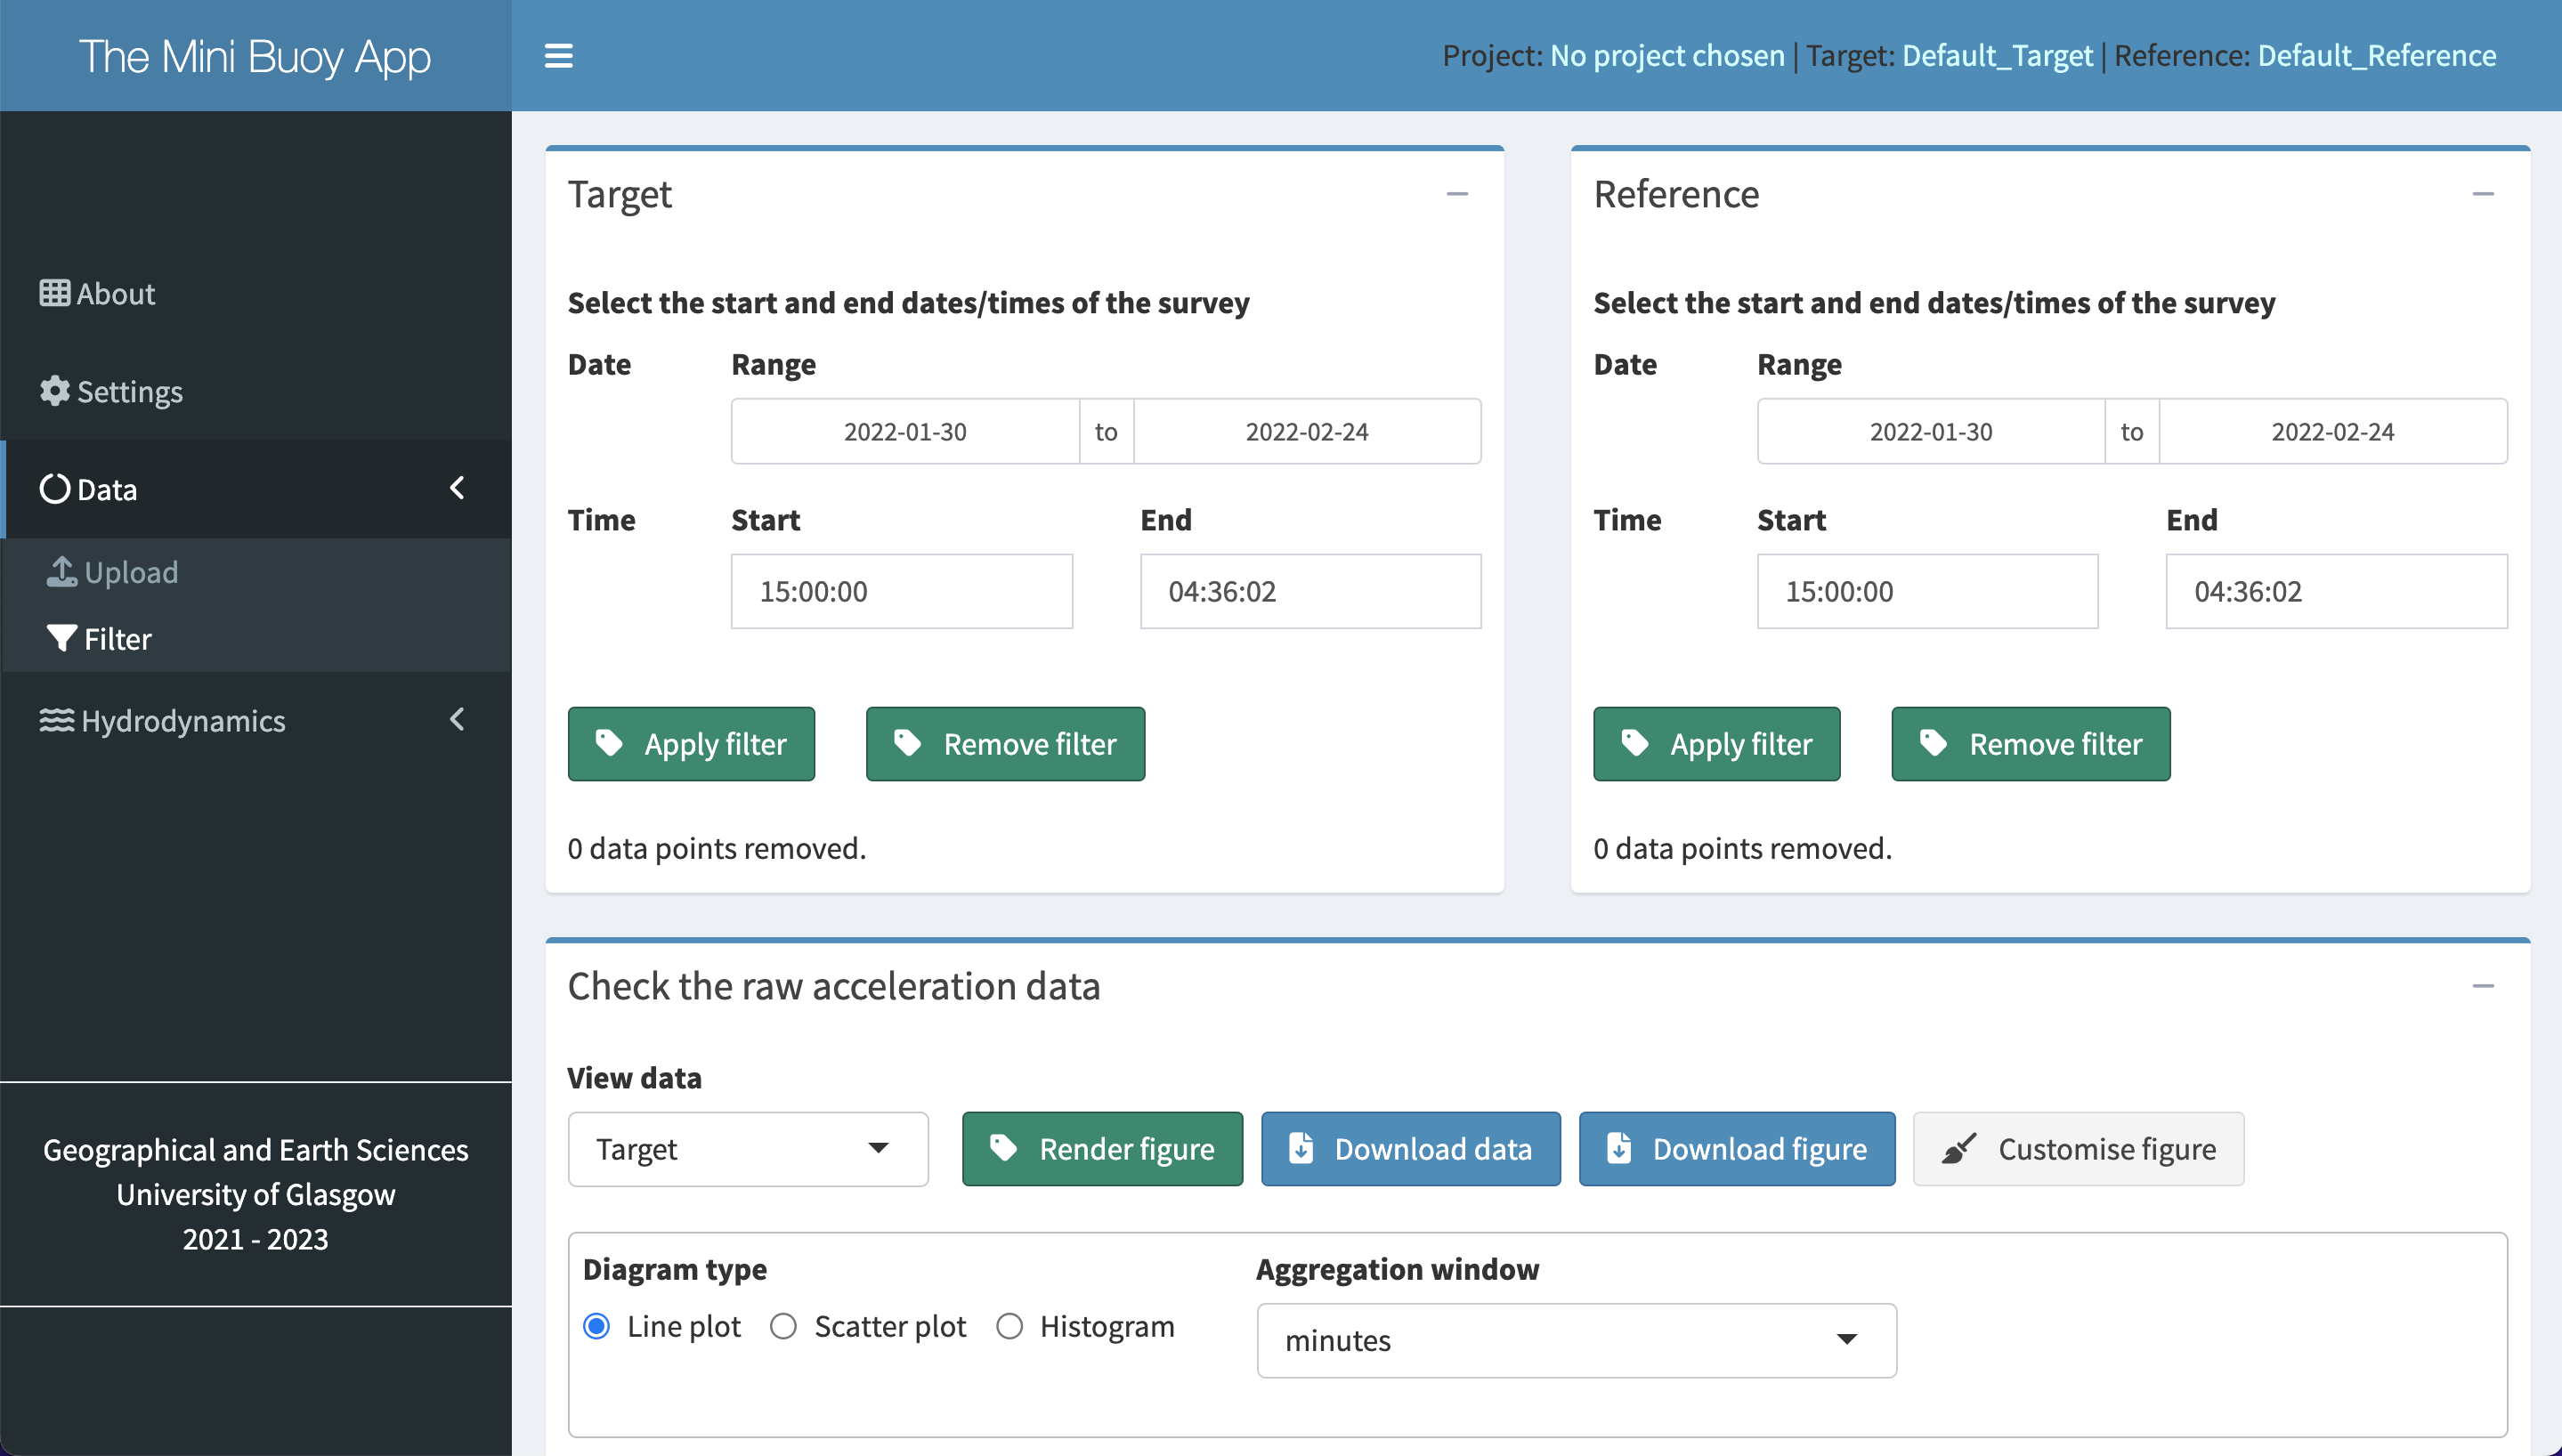
\includegraphics[width=1\textwidth,height=\textheight]{chapters/figs/DataFilter.png}

}

\end{figure}

\hypertarget{hydrodynamics}{%
\subsection{Hydrodynamics}\label{hydrodynamics}}

Inundation, current velocity, and wave orbital velocity (if B4+ Mini
Buoy is used) statistics are generated and presented automatically.
Users are helped with interpreting the results via a text summary,
tabulated data, and figure outputs. Users can interact with the figures
and download a comprehensive tabulated data that includes the raw
results. By modifying custom settings, users may seek to improve
inundation status classification and thereby current/wave metrics should
the default parameters be unsatisfactory.

\begin{enumerate}
\def\labelenumi{\arabic{enumi}.}
\tightlist
\item
  Select \texttt{Hydrodynamics} and \texttt{Target} or
  \texttt{Reference} from the left-hand menu, and wait for the App to
  analyse the data. Analysis is based on the default custom settings
  shown under the \texttt{Custom\ settings} drop-down window.
\item
  Inspect the summary text, table, and figures to assess the quality of
  the analysis, and amend the \texttt{Custom\ settings} if necessary
  (see Section~\ref{sec-custom}).
\item
  Select \texttt{Download\ results} and \texttt{Download\ plots} to save
  copies of the data and figures respectively. Further explanation of
  each below.
\item
  For a comparison between \texttt{Target} and \texttt{Reference} sites,
  select \texttt{Comparison} from the left-hand menu. Analysis is based
  on the default custom settings as specified under the
  \texttt{Custom\ settings} drop-down window for both \texttt{Target}
  and \texttt{Reference} menus.
\end{enumerate}

\begin{tcolorbox}[enhanced jigsaw, bottomrule=.15mm, leftrule=.75mm, bottomtitle=1mm, breakable, opacityback=0, colback=white, left=2mm, toprule=.15mm, opacitybacktitle=0.6, arc=.35mm, colframe=quarto-callout-note-color-frame, toptitle=1mm, titlerule=0mm, colbacktitle=quarto-callout-note-color!10!white, coltitle=black, title=\textcolor{quarto-callout-note-color}{\faInfo}\hspace{0.5em}{Note}, rightrule=.15mm]

Given that only the B4+ Mini Buoy measures wave orbital velocity, no
statistics for wave orbital velocity will be generated when other Mini
Buoy designs are used.

\end{tcolorbox}

\begin{figure}

{\centering 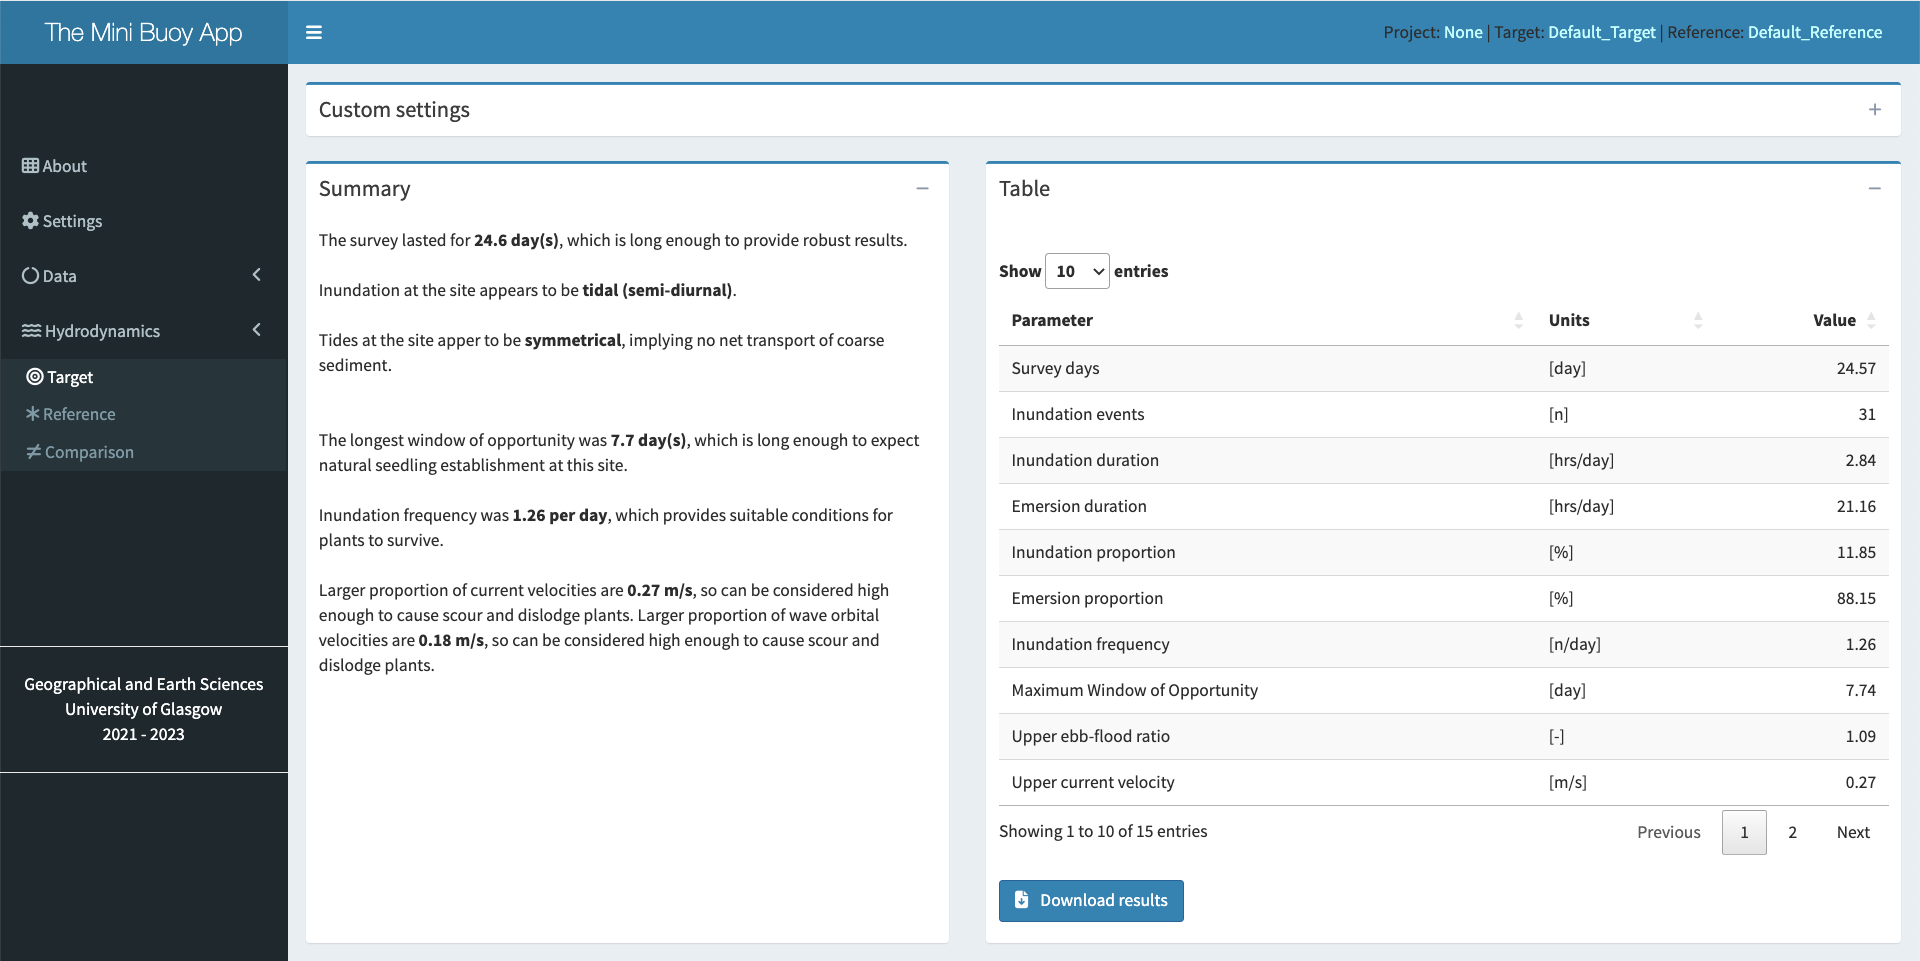
\includegraphics[width=1\textwidth,height=\textheight]{chapters/figs/HydroSingle.png}

}

\end{figure}

\hypertarget{sec-custom}{%
\subsubsection{Custom settings}\label{sec-custom}}

Custom settings determine how the App cleans inundation classifications
to achieve optimal results. Whilst the default settings are sufficient
in most cases, some sites may experience unique tidal characteristics
that require a tuning of the \texttt{Custom\ settings}. Having a
reliable classification of inundation is necessary for the next step of
calculating current and wave orbital velocities reliably. See
\textbf{TROUBLESHOOTING TBC} for examples of what to look out for in the
raw data that indicates the default settings may need changing. There
are four parameters that users can tune:

\begin{itemize}
\tightlist
\item
  \textbf{Minimum gap.} Occasionally, the App will misclassify clusters
  of points during an inundation event as ``non inundated''. This tends
  to happen during periods when there's a strong, consistent current (a
  signal that can be indistinguishable from a Mini Buoy lying at rest).
  Slight wobbling in the Mini Buoy does allow the App to classify the
  majority of the inundation event correctly. For the cluster of points
  are are wrongly classified as ``non-inundated'', the App will
  reclassify these according to the \texttt{Minimum\ gap} argument, that
  says ``any cluster shorter than this time window will be classified as
  fully inundated''. It is important that the \texttt{Minimum\ gap}
  argument is less than the time between inundation events - otherwise,
  the gap between two tides will be classed as ``fully inundated''!
\item
  \textbf{Search window.} The start and end of each inundation event is
  initially classified as ``fully inundated'' by the App. Since a
  partially inundated Mini Buoy will give the same signal as one that's
  fully submerged and being pushed by a strong current, it is important
  to distinguish between these. The App identifies partially inundated
  cases during flood tide by looking for the abrupt shift in a Mini Buoy
  moving from a horizontal position (\textasciitilde0°) to a near
  vertical one (near 90°) before any current may start pushing against
  it (moving towards 0° again). The reverse pattern applies for ebb
  tides. This is done by identifying the first and last timestamp of a
  given inundation event, and then searching for abrupt shifts before
  and after these points over a specified time window. The time window
  is defined by the \texttt{Search\ window} argument, which is a
  proportion of each inundation event. For example, a value of 25\%
  means that the search window is quarter the length of a given
  inundation event. The middle of the search window is placed at the
  start and end of the event, so that 12.5\% of the search window before
  and after are used in searching for abrupt shifts around the start and
  end of inundation events. The maximum amount of data that can be used
  is 50\% (i.e., the full flood and ebb tide lengths). A longer search
  window will result in a more conservative classification, so that
  fully inundated cases may be classified as partially inundated.
  Shorter inundation windows may help capture peak flood/ebb tides,
  though also increases the probability of missing truly partially
  inundated cases.
\item
  \textbf{Minimum duration.} Some flooding events, especially nearer
  neap tides, may result in only very short periods of inundation.
  Taking current and wave orbital velocities from these events may be
  unwise, especially if the Mini Buoy is only just fully submerged.
  \texttt{Minimum\ duration} sets the minimum duration of inundation
  that an event needs to be in order to be used in the analysis.
  Anything below this threshold is classified as partially inundated.
\item
  \textbf{Minimum tilt.} Some flooding events may be too shallow to
  raise the Mini Buoy to a fully upright position (90°) as would be
  expected during slack water. In such cases, current and wave orbital
  velocity values may be spurious. \texttt{Minimum\ tilt} specifies the
  minimum tilt that needs to be crossed per inundation event, otherwise
  the entire event is classified as partially inundated. Note, if a site
  is exposed to currents throughout the survey, the Mini Buoy may never
  reach 90°. This is why specifying a custom \texttt{Minimum\ tilt}
  appropriate to the study area in question may help improve results.
\end{itemize}

Examples are given in the \textbf{TROUBLESHOOT TBC} chapter to help
users identify where issues may be occurring and how to remedy them. It
can be good practice to modify the \texttt{Custom\ settings} and see
what effect that has on the results - which may be negligible.

\begin{figure}

{\centering 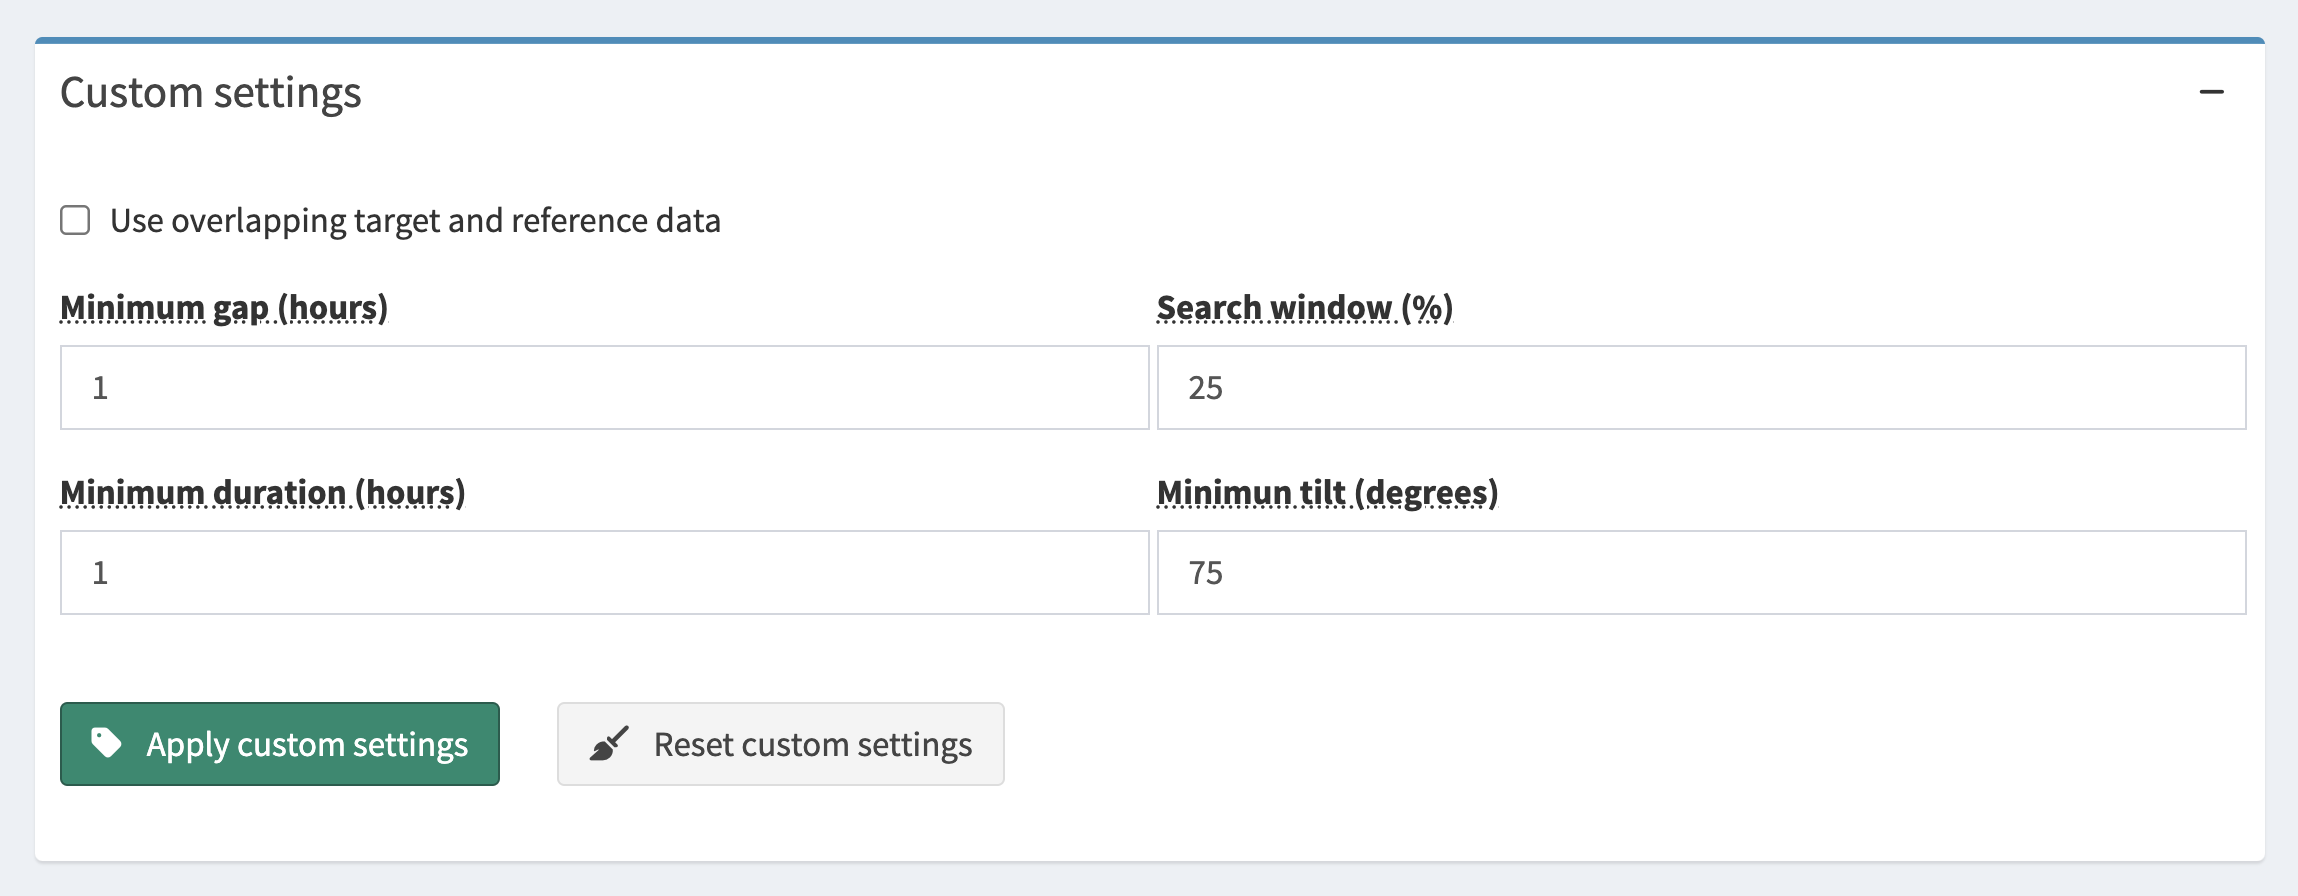
\includegraphics[width=1\textwidth,height=\textheight]{chapters/figs/CustomSettings.png}

}

\end{figure}

\hypertarget{summary}{%
\subsubsection{Summary}\label{summary}}

The summary text provides a simple language overview of key results, to
ascertain whether the site is generally suitable for the natural or
managed establishment of coastal vegetation. Indications of whether the
site is suitable for restoration are given, depending on the length of
the survey, the type and symmetry of the tidal regime, duration of the
longest inundation-free period (i.e., Window of Opportunity for seedling
establishment), inundation frequency, exposure to current velocity, and
exposure to wave orbital velocity (if the B4+ design is used). For
example, a site may have low current and wave exposure (that suit
restoration) but excessive inundation duration (that hamper
restoration).

\hypertarget{figures}{%
\subsubsection{Figures}\label{figures}}

\section{Raw data}

\begin{figure}

{\centering 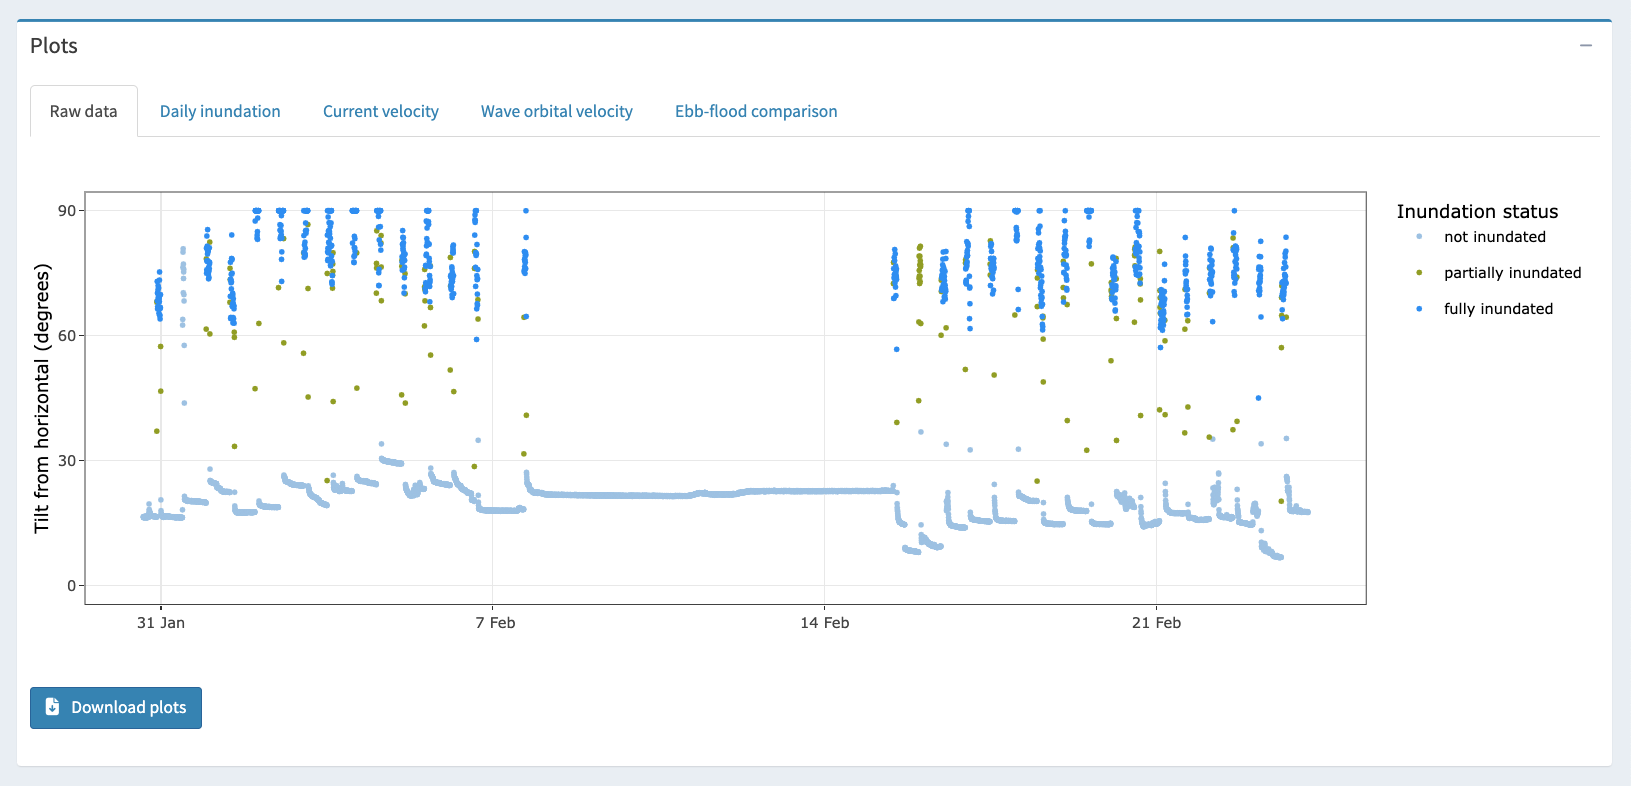
\includegraphics[width=1\textwidth,height=\textheight]{chapters/figs/RawData.png}

}

\caption{Tilt of the Mini Buoy over time, colour-coded to show the
inundation status (non/partial/full) as classified by the App. This plot
is a useful check to confirm whether the classification was successful
(see Section~\ref{sec-custom})}

\end{figure}

\section{Daily inundation}

\begin{figure}

{\centering 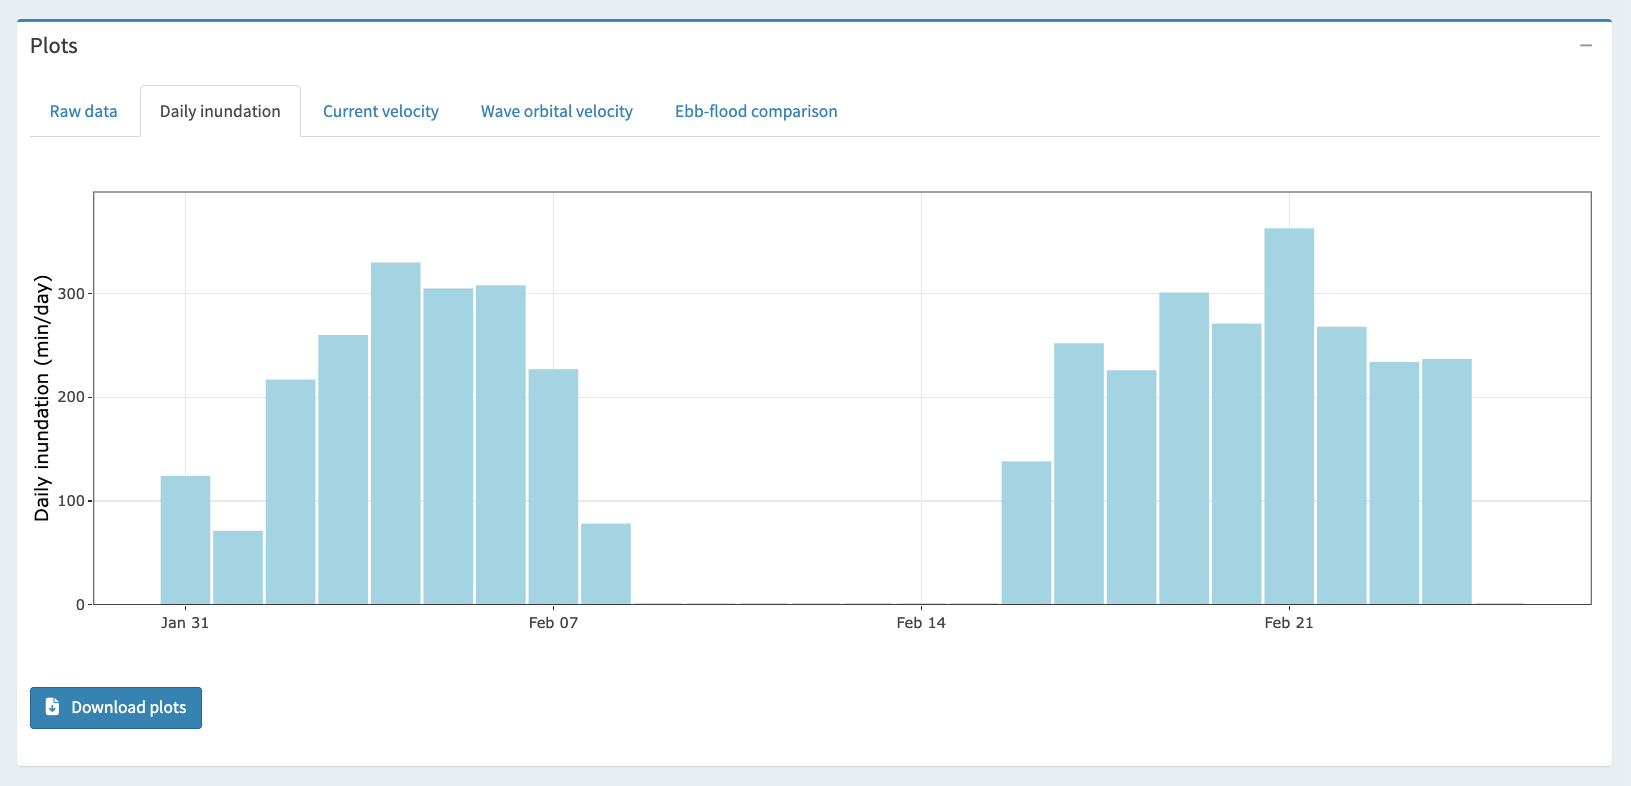
\includegraphics[width=1\textwidth,height=\textheight]{chapters/figs/InundationData.png}

}

\caption{Daily inundation duration per day. Spring/neap tidal cycles and
periods of emersion (no inundation) can be easily detected.}

\end{figure}

\section{Current velocity}

\begin{figure}

{\centering 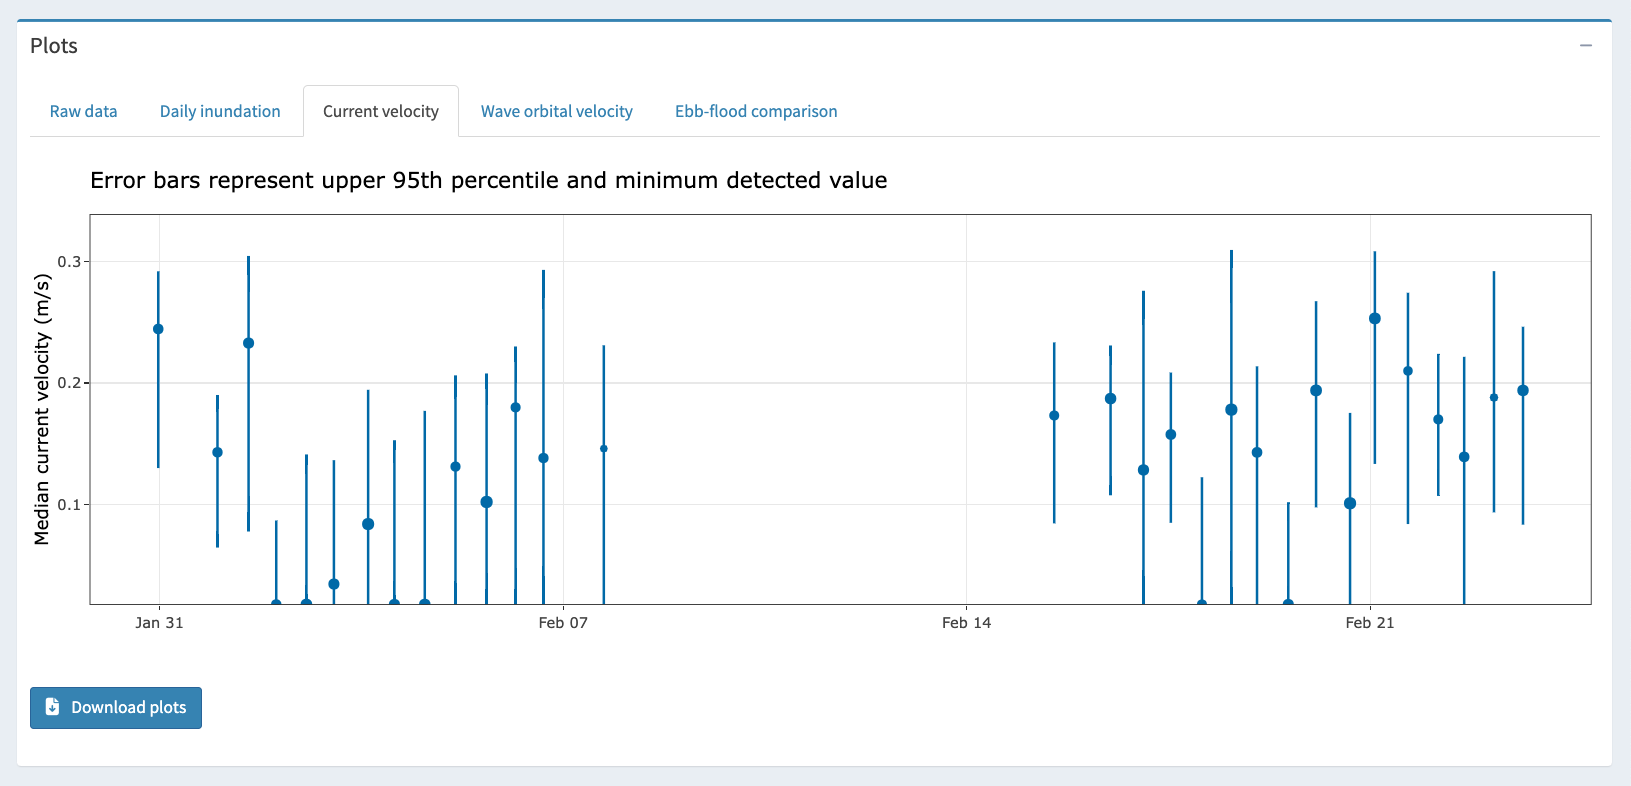
\includegraphics[width=1\textwidth,height=\textheight]{chapters/figs/CurrentsData.png}

}

\caption{Current velocities per day. The point represents median values
per day, and the size of the points is scaled to the number of
inundation events per day (the larger the point, the more inundation
events there were). The top error bar represents the largest velocities
(expressed as the upper 95th percentile of velocities) whilst the bottom
error bar represents the smallest velocities detected per day.}

\end{figure}

\section{Wave orbital velocity}

\begin{figure}

{\centering 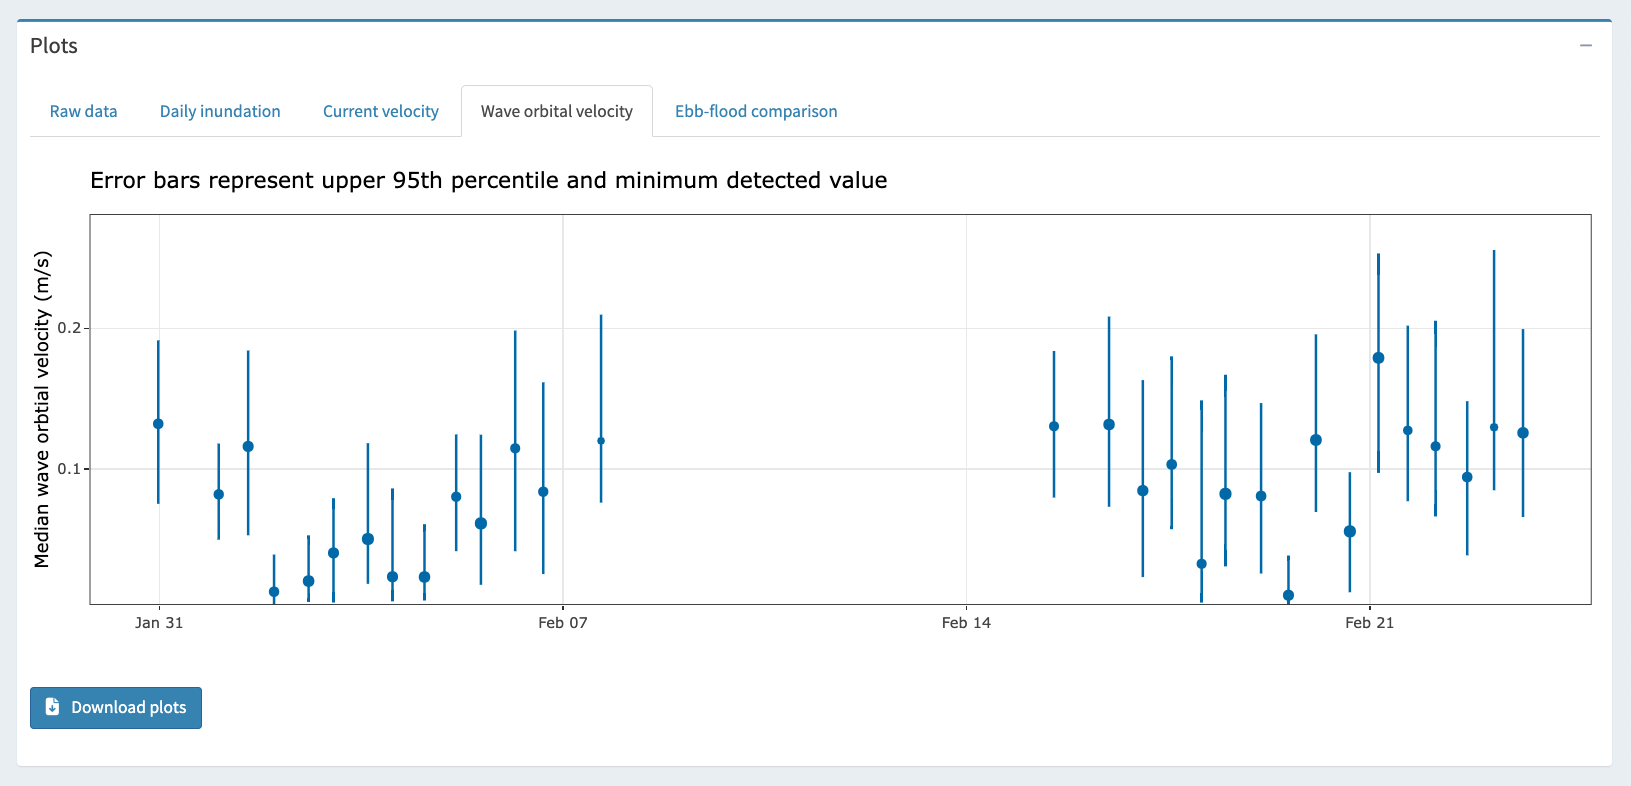
\includegraphics[width=1\textwidth,height=\textheight]{chapters/figs/WaveData.png}

}

\caption{Wave orbital velocities per day. The point represents median
values per day, and the size of the points is scaled to the number of
inundation events per day (the larger the point, the more inundation
events there were). The top error bar represents the largest velocities
(expressed as the upper 95th percentile of velocities) whilst the bottom
error bar represents the smallest velocities detected per day.}

\end{figure}

\section{Ebb-flood comparison}

\begin{figure}

{\centering 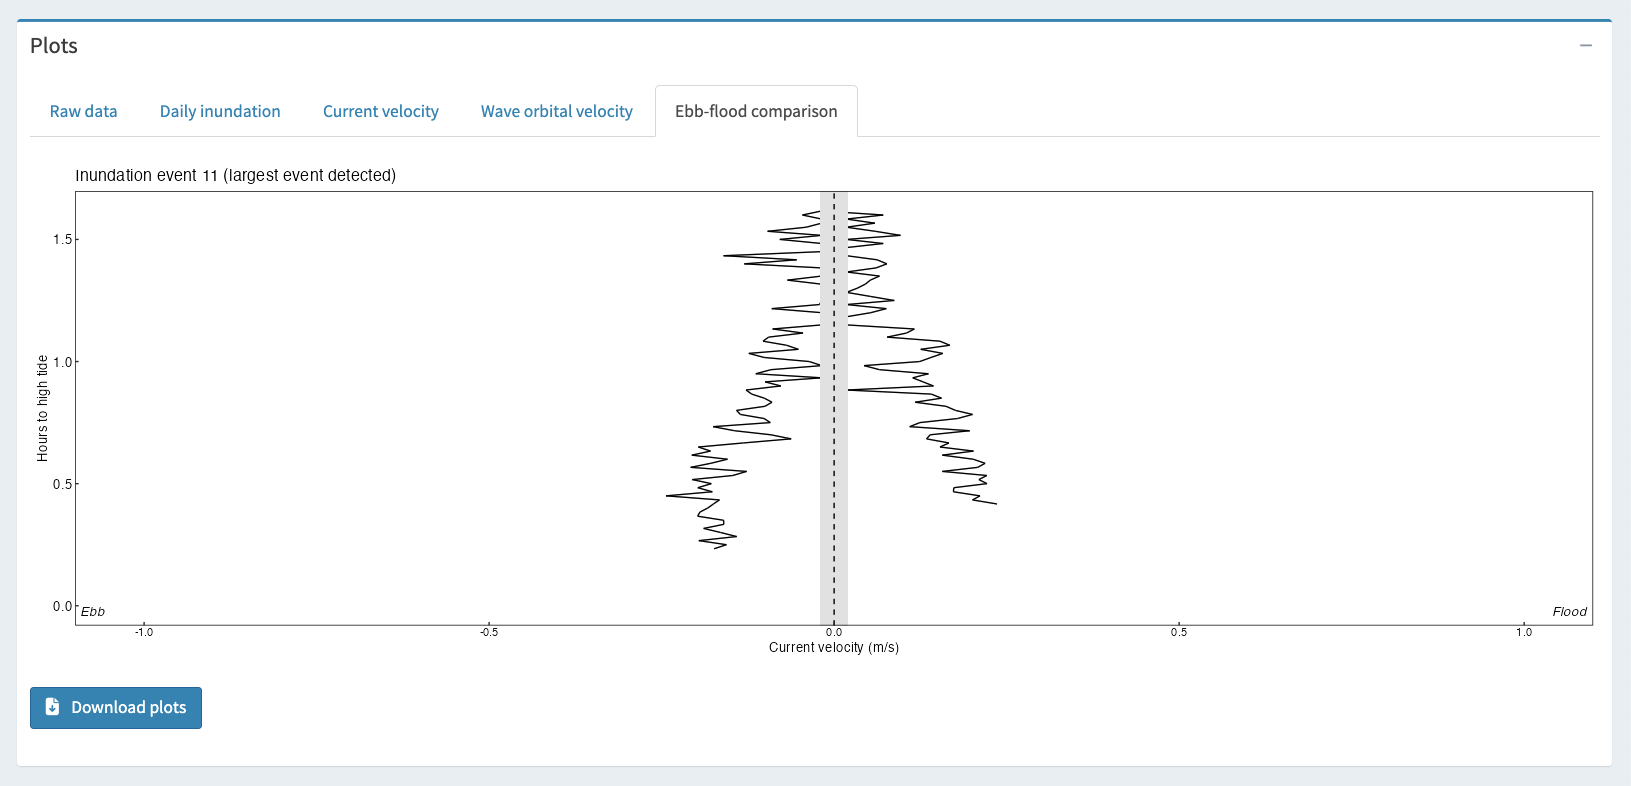
\includegraphics[width=1\textwidth,height=\textheight]{chapters/figs/EbbFloodData.png}

}

\caption{Timing of current velocities for the ebb (expressed with
negative values) and flood (expressed with positive values) to/from high
tide (slack water) for the longest inundation event detected by the App.
This is a useful way to determine whether the may be any asymmetry in
the tide (e.g., flood dominance where the duration of inundation on the
flood tide is shorter and has larger currents), which has implications
for the direction of net sediment transport.}

\end{figure}

\bookmarksetup{startatroot}

\hypertarget{references}{%
\chapter*{References}\label{references}}
\addcontentsline{toc}{chapter}{References}

\markboth{References}{References}

\hypertarget{refs}{}
\begin{CSLReferences}{0}{0}
\end{CSLReferences}



\end{document}
